% Include Preamble 
\documentclass[10pt,dvipsnames, aspectratio=169]{beamer}
\usetheme[progressbar=frametitle]{metropolis}
\usepackage[]{verbatim}\usepackage[]{}
\usepackage{booktabs}
\usepackage[scale=2]{ccicons}
\usepackage[misc]{ifsym}
\usepackage{wasysym}
\usepackage{listings}
\usepackage{xspace}
\usepackage{amsmath}
\usepackage{xcolor}
\usepackage{ragged2e}\justifying % for justify content % Customize 
\setlength{\parskip}{5pt} % vertical spacing between 2 paragraphs
\setbeamersize{text margin left=12mm, text margin right=12mm} 
\setbeamertemplate{frametitle}[default][left, leftskip=8mm]
%\usepackage[hidelink]{hyperref}
\newcommand{\themename}{\textbf{\textsc{metropolis}}\xspace}

% WARNING: Don't Touch,if you are not compfortable! 
\addtobeamertemplate{frametitle}{}{
%\begin{tikzpicture}[remember picture,overlay]
%\node[anchor=north east,yshift=2pt,xshift=-65pt] at (current page.north east) 
%{\includegraphics[height=.75cm]{img/elixir-portugal-white}};
%\node[anchor=north east,yshift=4pt] at (current page.north east) 
%{
\includegraphics[height=1cm]{img/hdro}};
%\end{tikzpicture}
}

% Title Page of Presentation 
% WARNING: Don't change logo, just write your details 
\title{Introduction to SPSS}
\date{\today}
\author{Md. Jubayer Hossain\\
        https://jhossain.me/}
\institute{Lead Organizer, Health Research ToolBox: A Step by Step Guide for Beginners 
\\ Founder,Center for Health Innovation, Research, Action, and Learning }
\titlegraphic{\vspace{4cm}\hfill
\includegraphics[height=1cm]{img/hdro2}}

\begin{document}
\maketitle
% Sectuion Title 
\section{SECTION--I Introduction}
% Slide 
\begin{frame}[t]{Opening a Data File (Con..)}
      \textbf{To open a data file:}\\
      	From the menus choose:\\
      	File \textgreater Open \textgreater Data..\\
\end{frame}
% Slide 
\begin{frame}[t]{Opening a Data File (Con..)}
		\begin{figure}
			\centering
			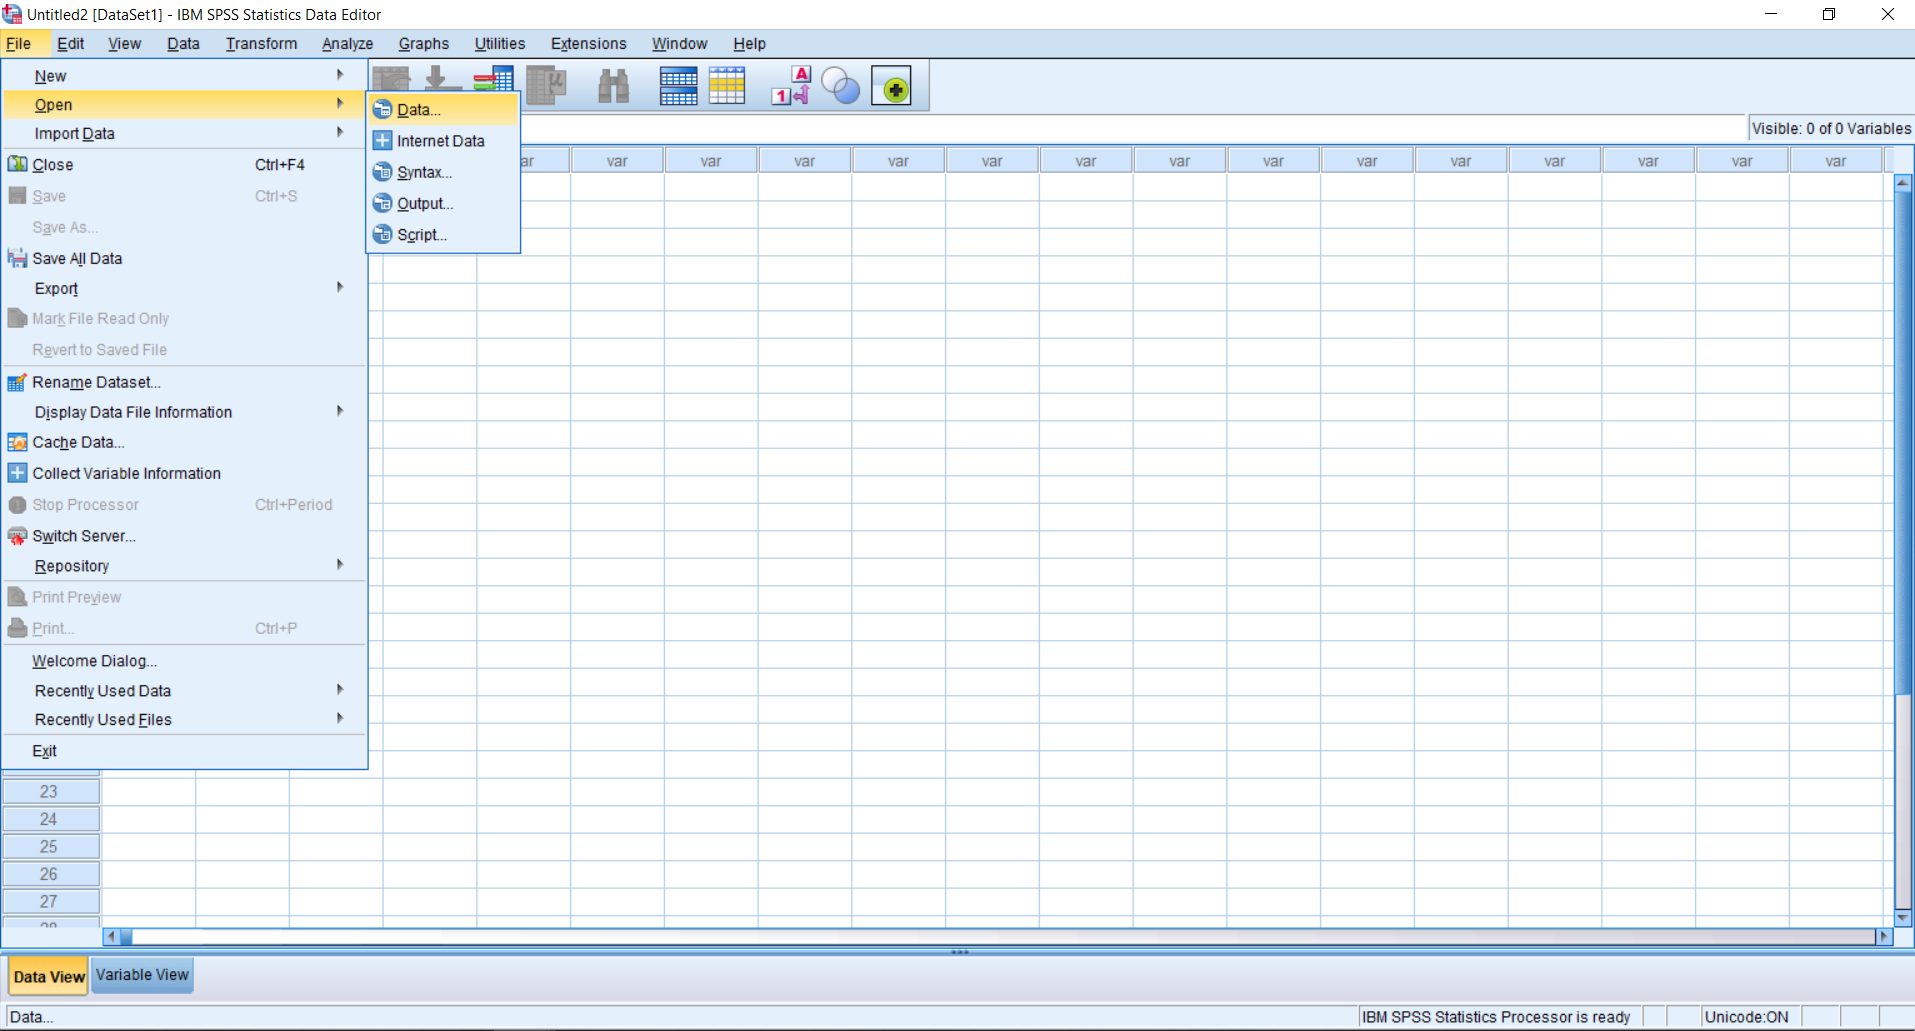
\includegraphics[width=12cm]{img/o_data_1}
			\caption{1st step}
		\end{figure}
\end{frame}
% Slide 
\begin{frame}[t]{Opening a Data File (Con..)}
		\begin{figure}
			\centering
			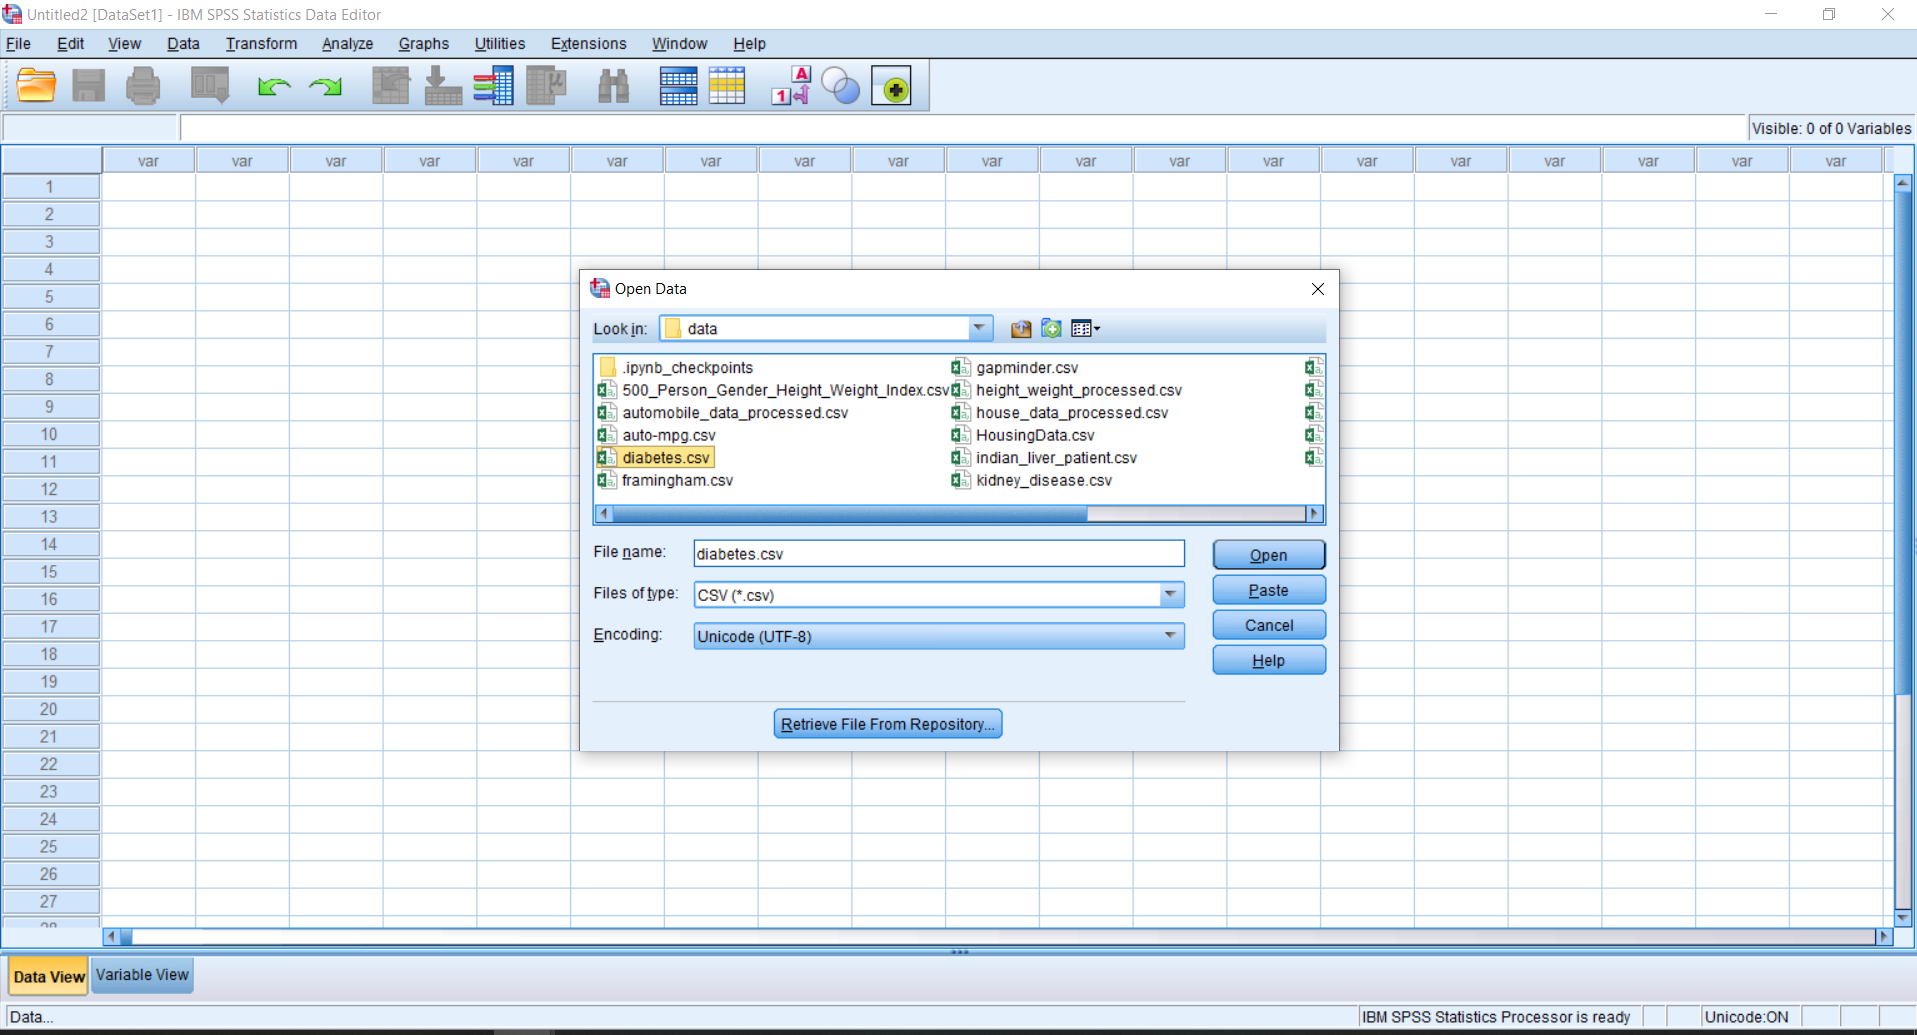
\includegraphics[width=12cm]{img/o_data_2}
			\caption{2nd step}
		\end{figure}
\end{frame}
% Slide 
\begin{frame}[t]{Opening a Data File}
		\begin{figure}
			\centering
			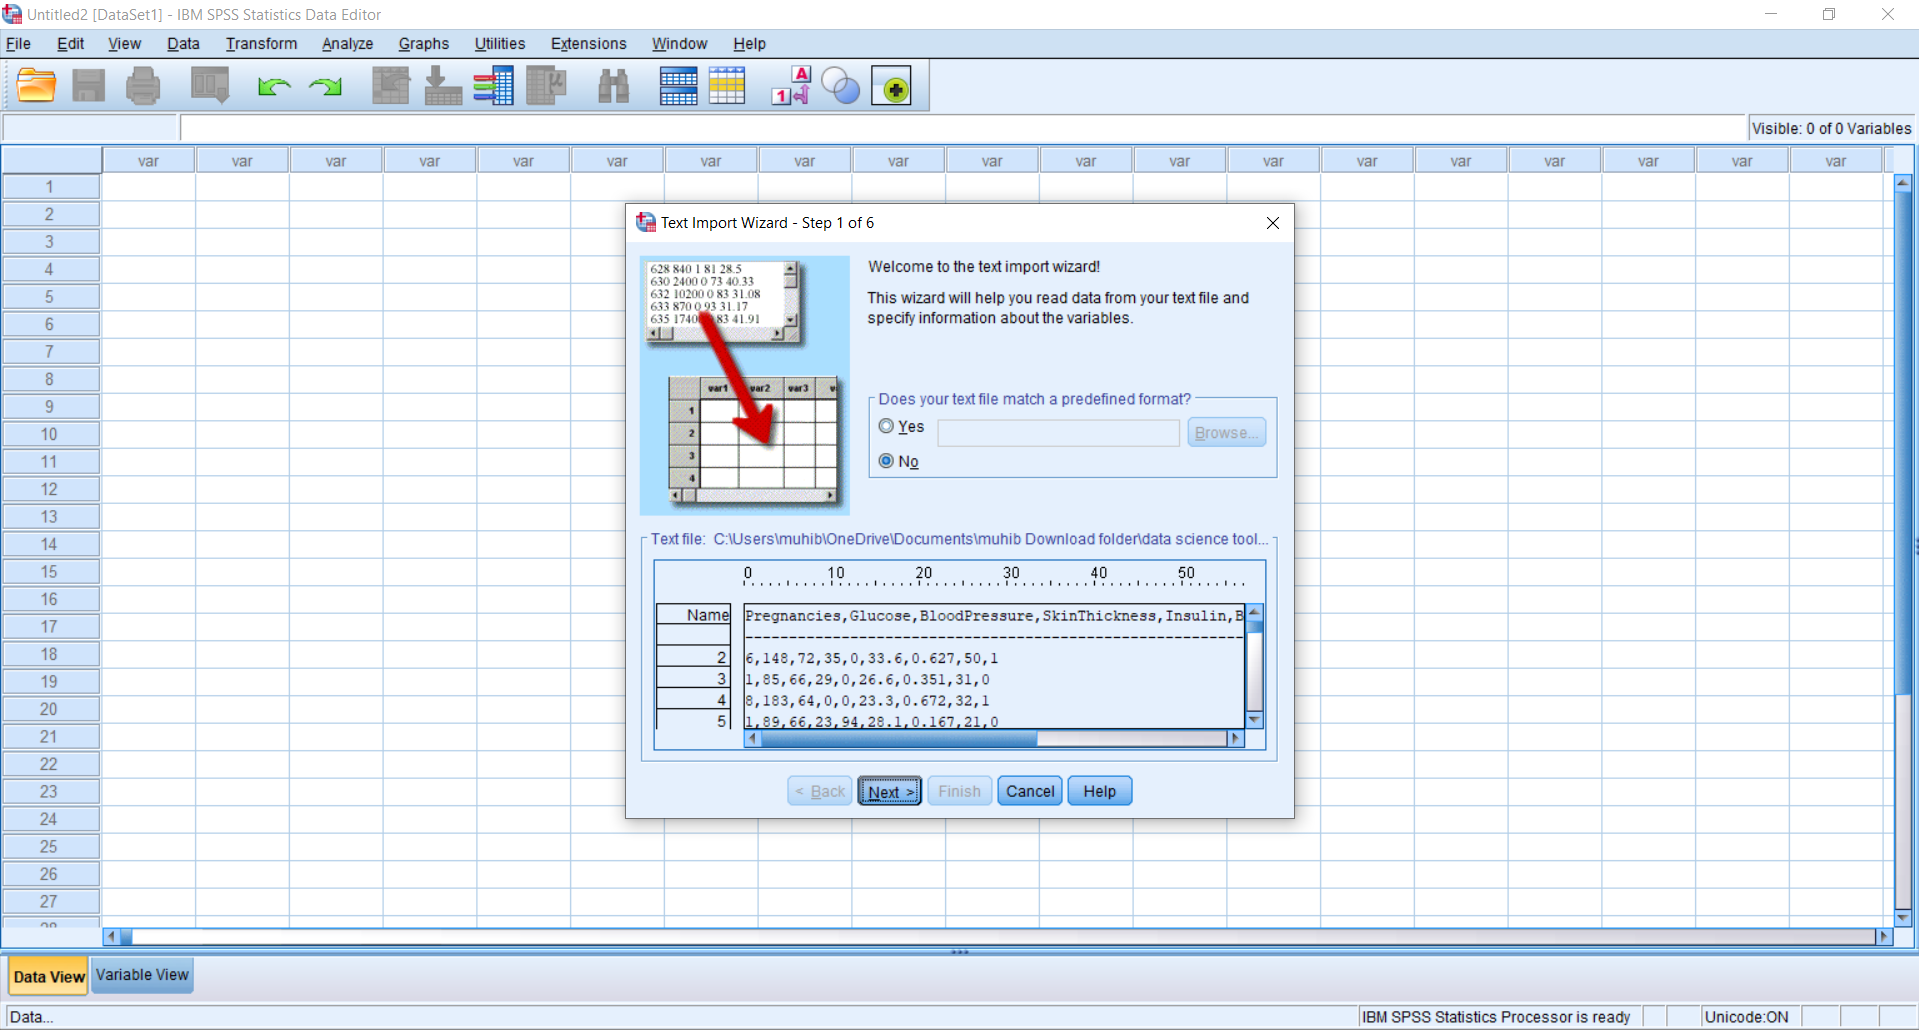
\includegraphics[width=12cm]{img/o_data_4}
			\caption{3rd step}
		\end{figure}
\end{frame}




%slide
\begin{frame}[t]{Running an Analysis (Con..)}
		\textbf{To run an analysis:}\\
		From the menus choose:\\
		Analyze \textgreater Descriptive Statistics \textgreater Frequencies...
\end{frame}
%slide
\begin{frame}[t]{Running an Analysis (Con..)}
		\begin{figure}
			\centering
			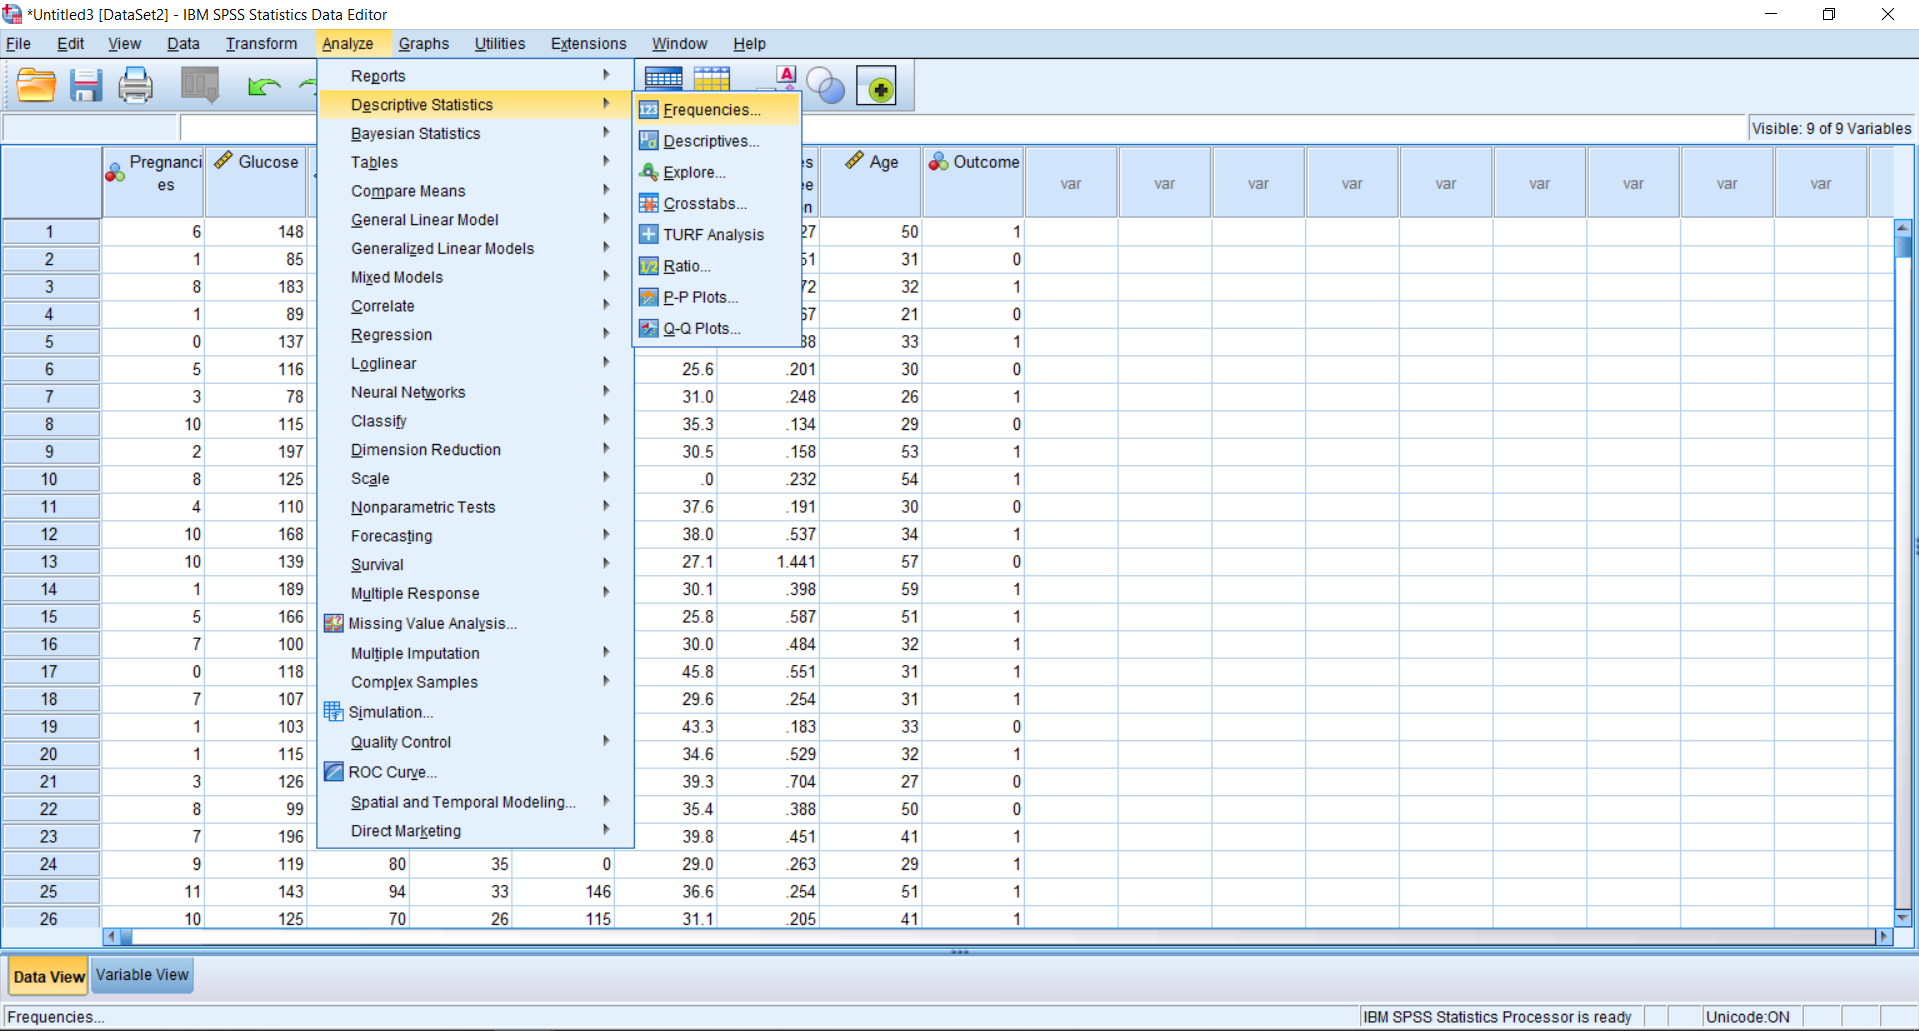
\includegraphics[width=12cm]{img/freq_table1}
			\caption{1st step}
		\end{figure}
\end{frame}
%slide
\begin{frame}[t]{Running an Analysis (Con..)}
		\begin{figure}
			\centering
			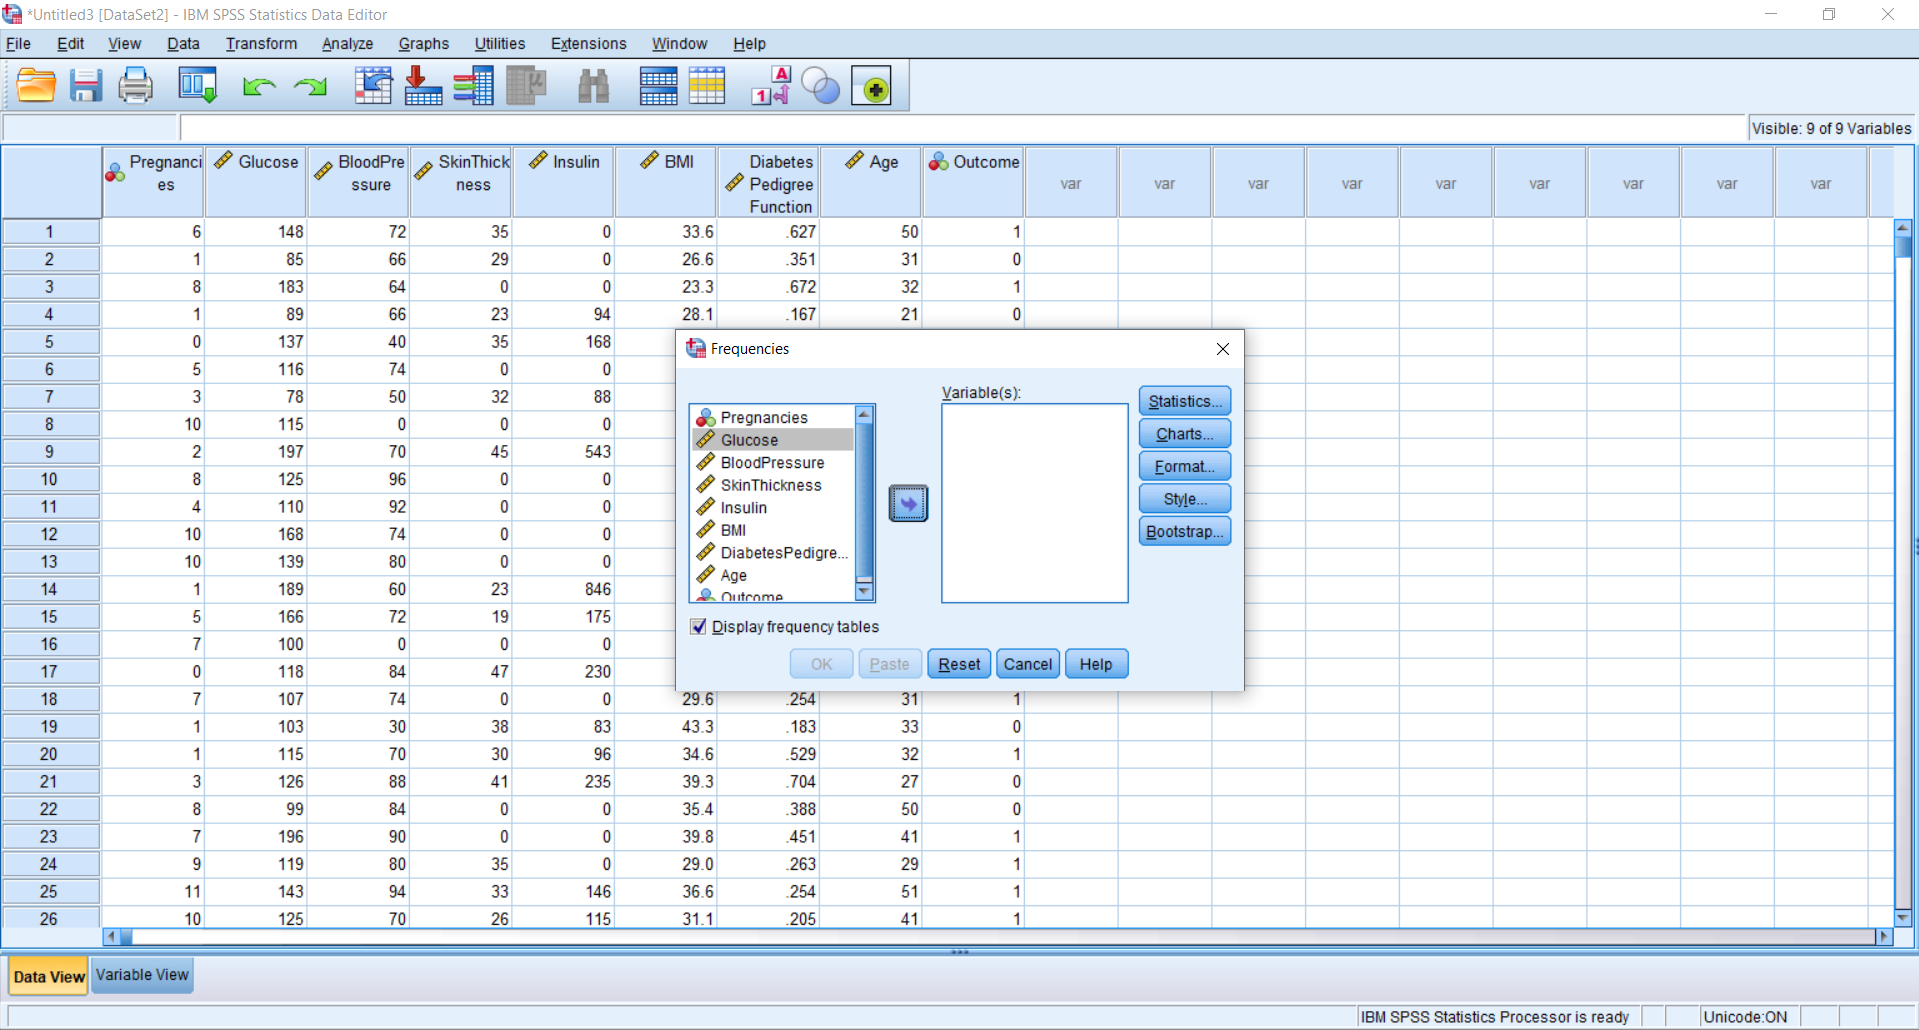
\includegraphics[width=12cm]{img/freq_table2}
			\caption{2nd step}
		\end{figure}	
\end{frame}
%slide
\begin{frame}[t]{Running an Analysis}
		\begin{figure}
			\centering
			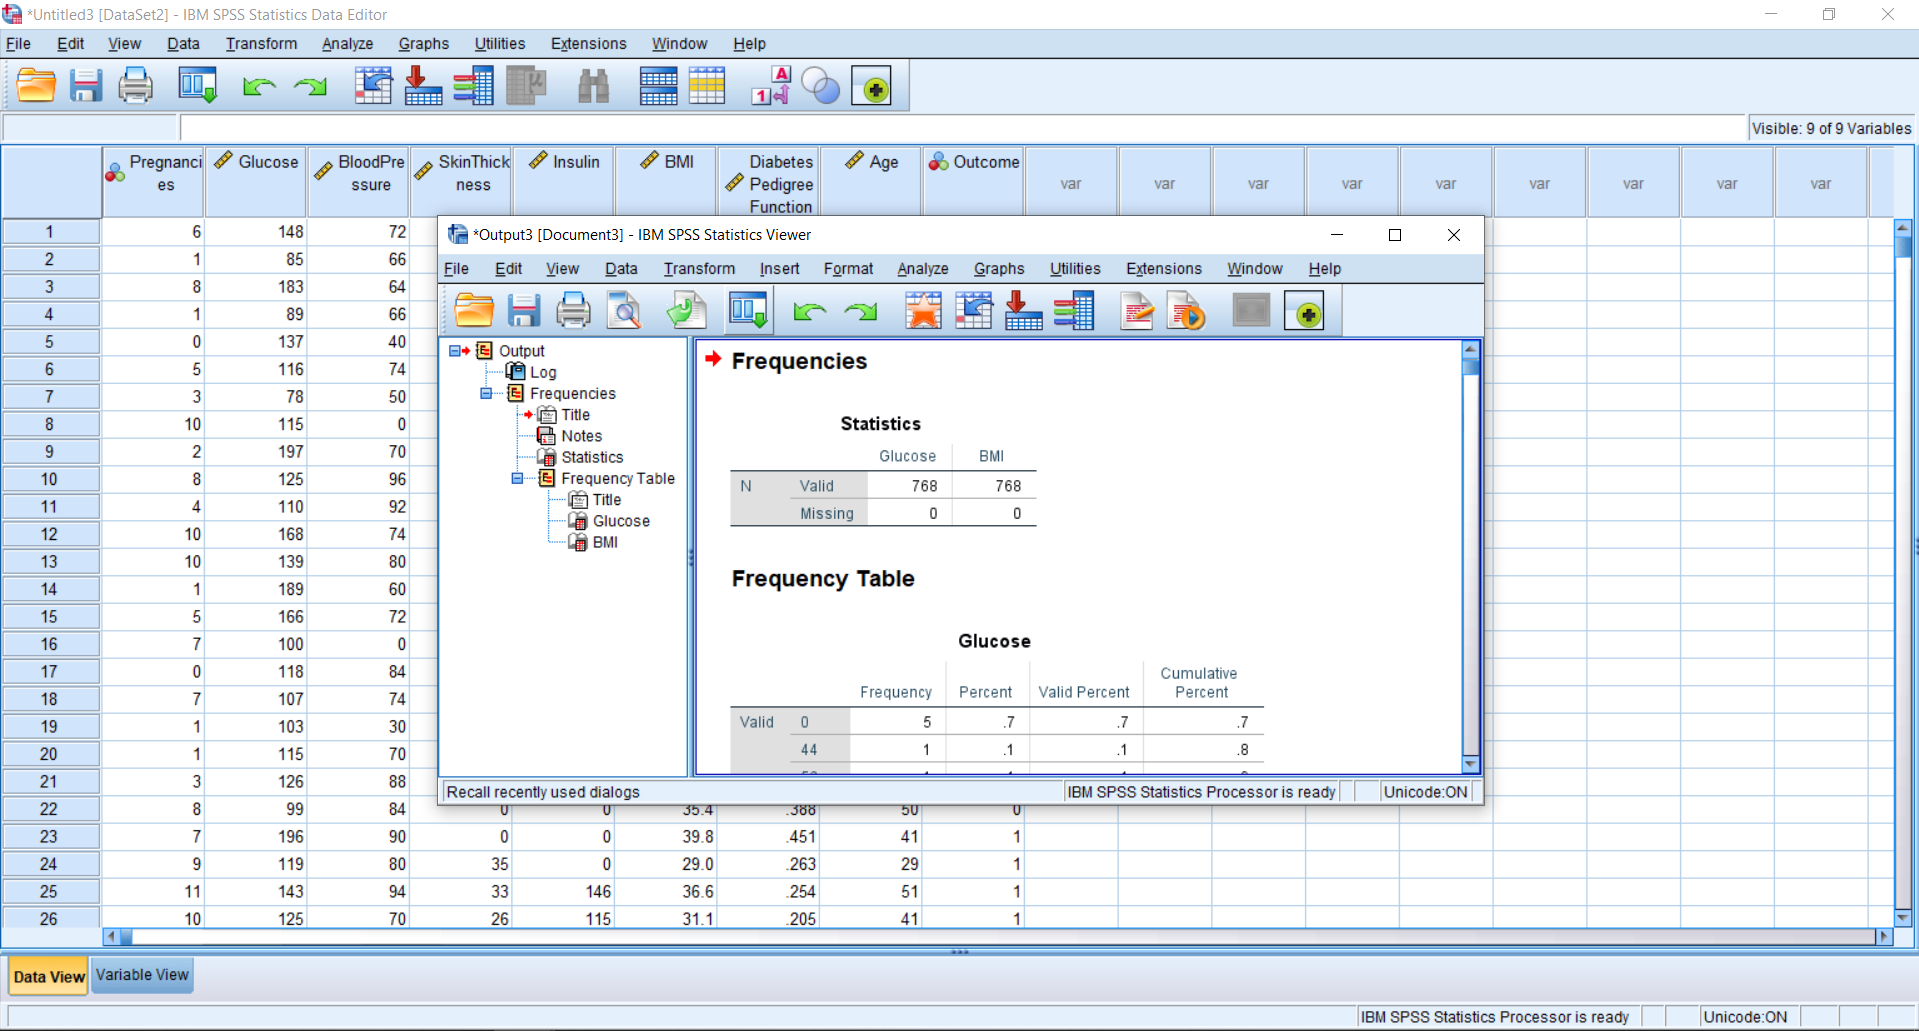
\includegraphics[width=12cm]{img/freq_table3}
			\caption{3rd step}
		\end{figure}
\end{frame}
%slide
\begin{frame}[t]{An icon next to each variable provides information about data type and level of measurement}
	\begin{figure}
		\centering
		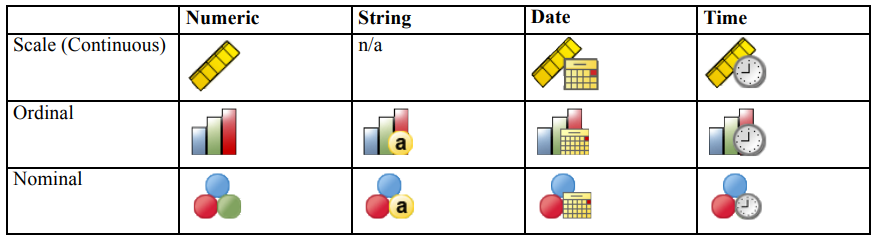
\includegraphics[width=12cm]{img/level_of_measurement}
		%\caption{3rd step}
	\end{figure}
\end{frame}

%slide
\begin{frame}[t]{Viewing Result}
	\begin{figure}
		\centering
		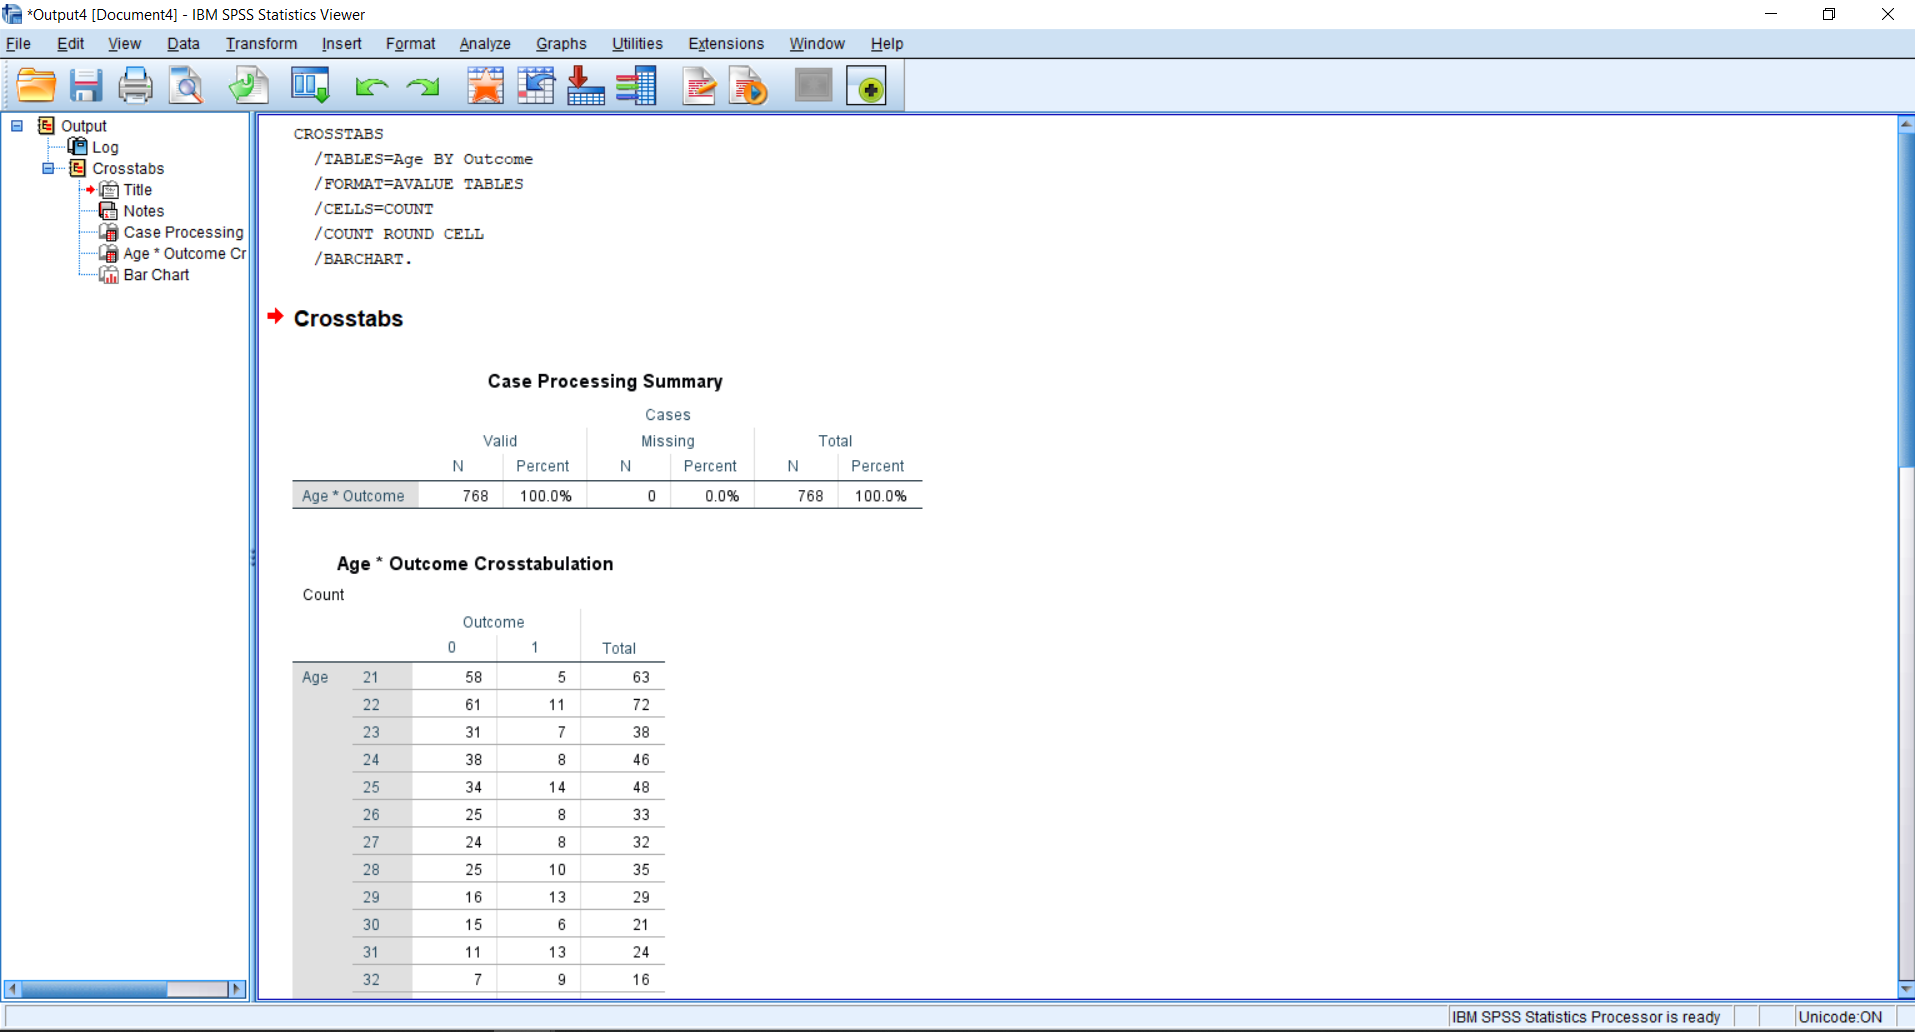
\includegraphics[width=12cm]{img/cross_table3}
		\caption{Result View}
	\end{figure}
\end{frame}
%slide
\begin{frame}[t]{Creating Charts (Con..)}
	\textbf{To create a chart:}\\
	From the menus choose:\\
	\begin{itemize}
	\item Graphs \textgreater Graph Template Chooser/ Legacy Dialogues...
	\item Click the Gallery tab (if it is not selected).
	\item Select Chart / variables (if it is not selected).
	\item Click OK to create the chart.
	\end{itemize}
\end{frame}
%slide
\begin{frame}[t]{Created Chart}
	\begin{figure}
		\centering
		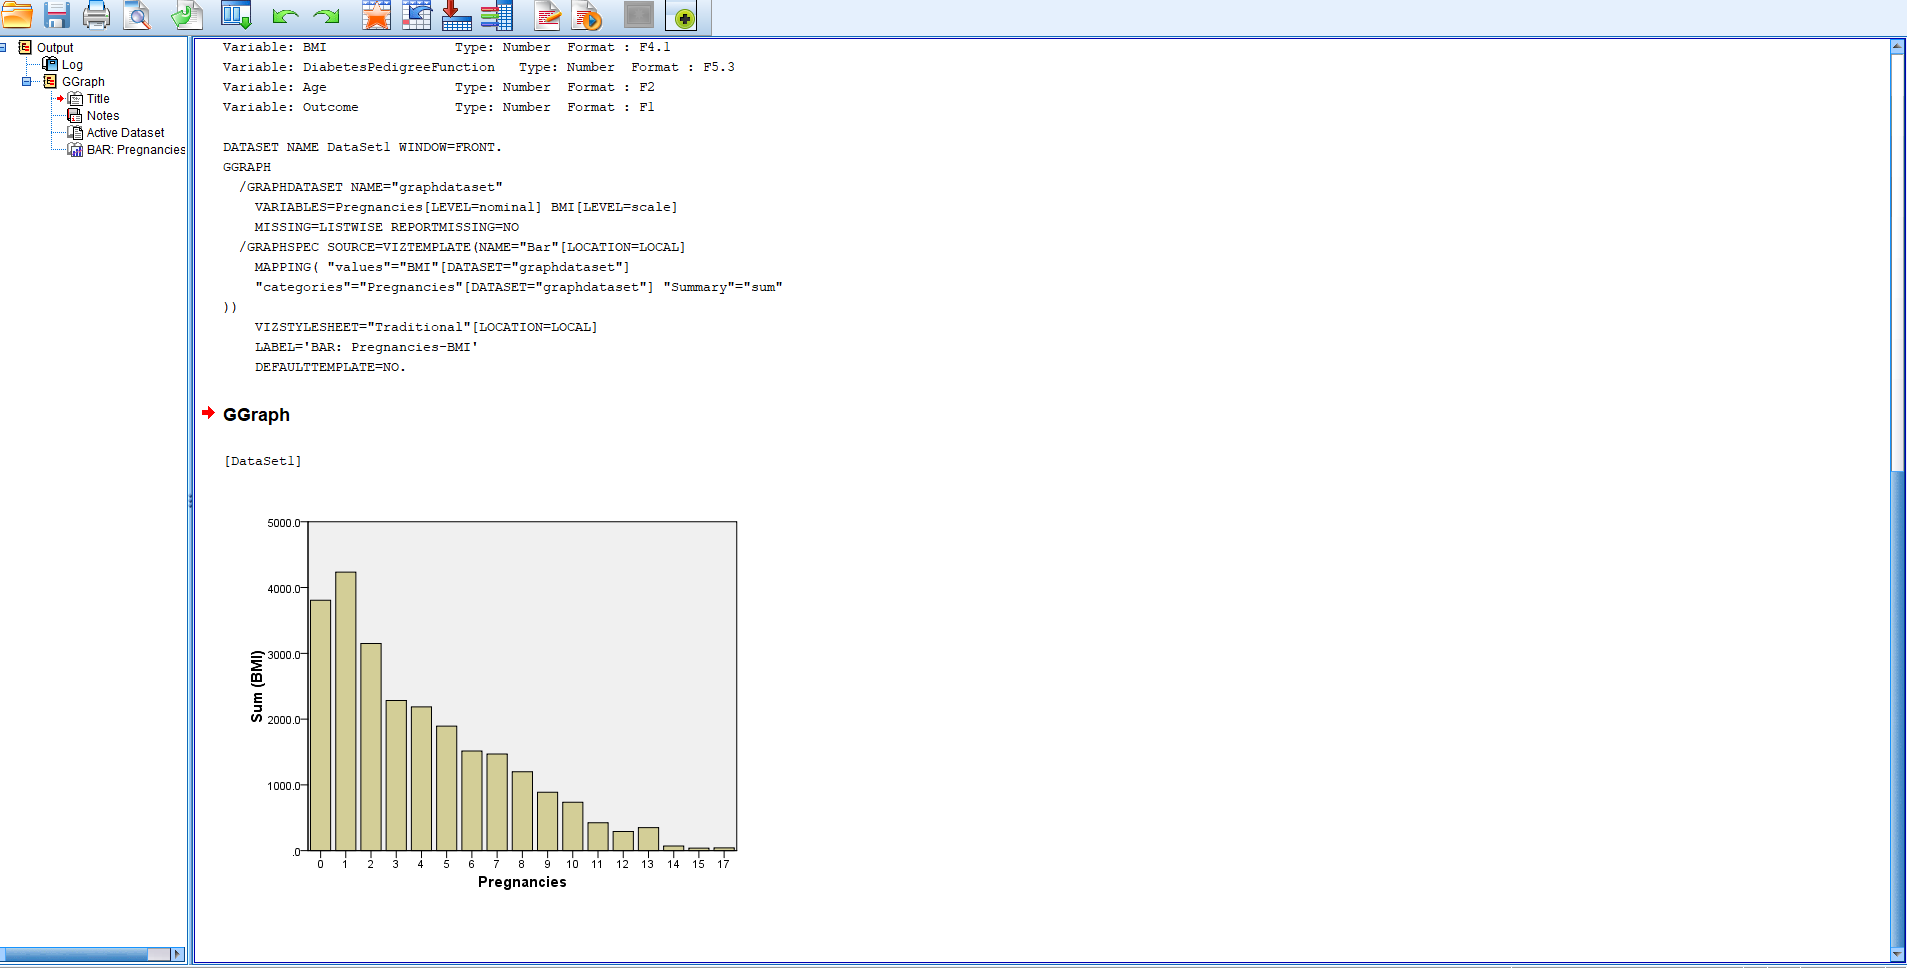
\includegraphics[width=12cm]{img/graph-1}
		\caption{Created Graph}
	\end{figure}
\end{frame}

% Sectuion Title 
\section{SECTION--II Reading Data}
%slide
\begin{frame}[t]{Basic Structure of IBM SPSS Statistics Data Files}
	\begin{figure}
		\centering
		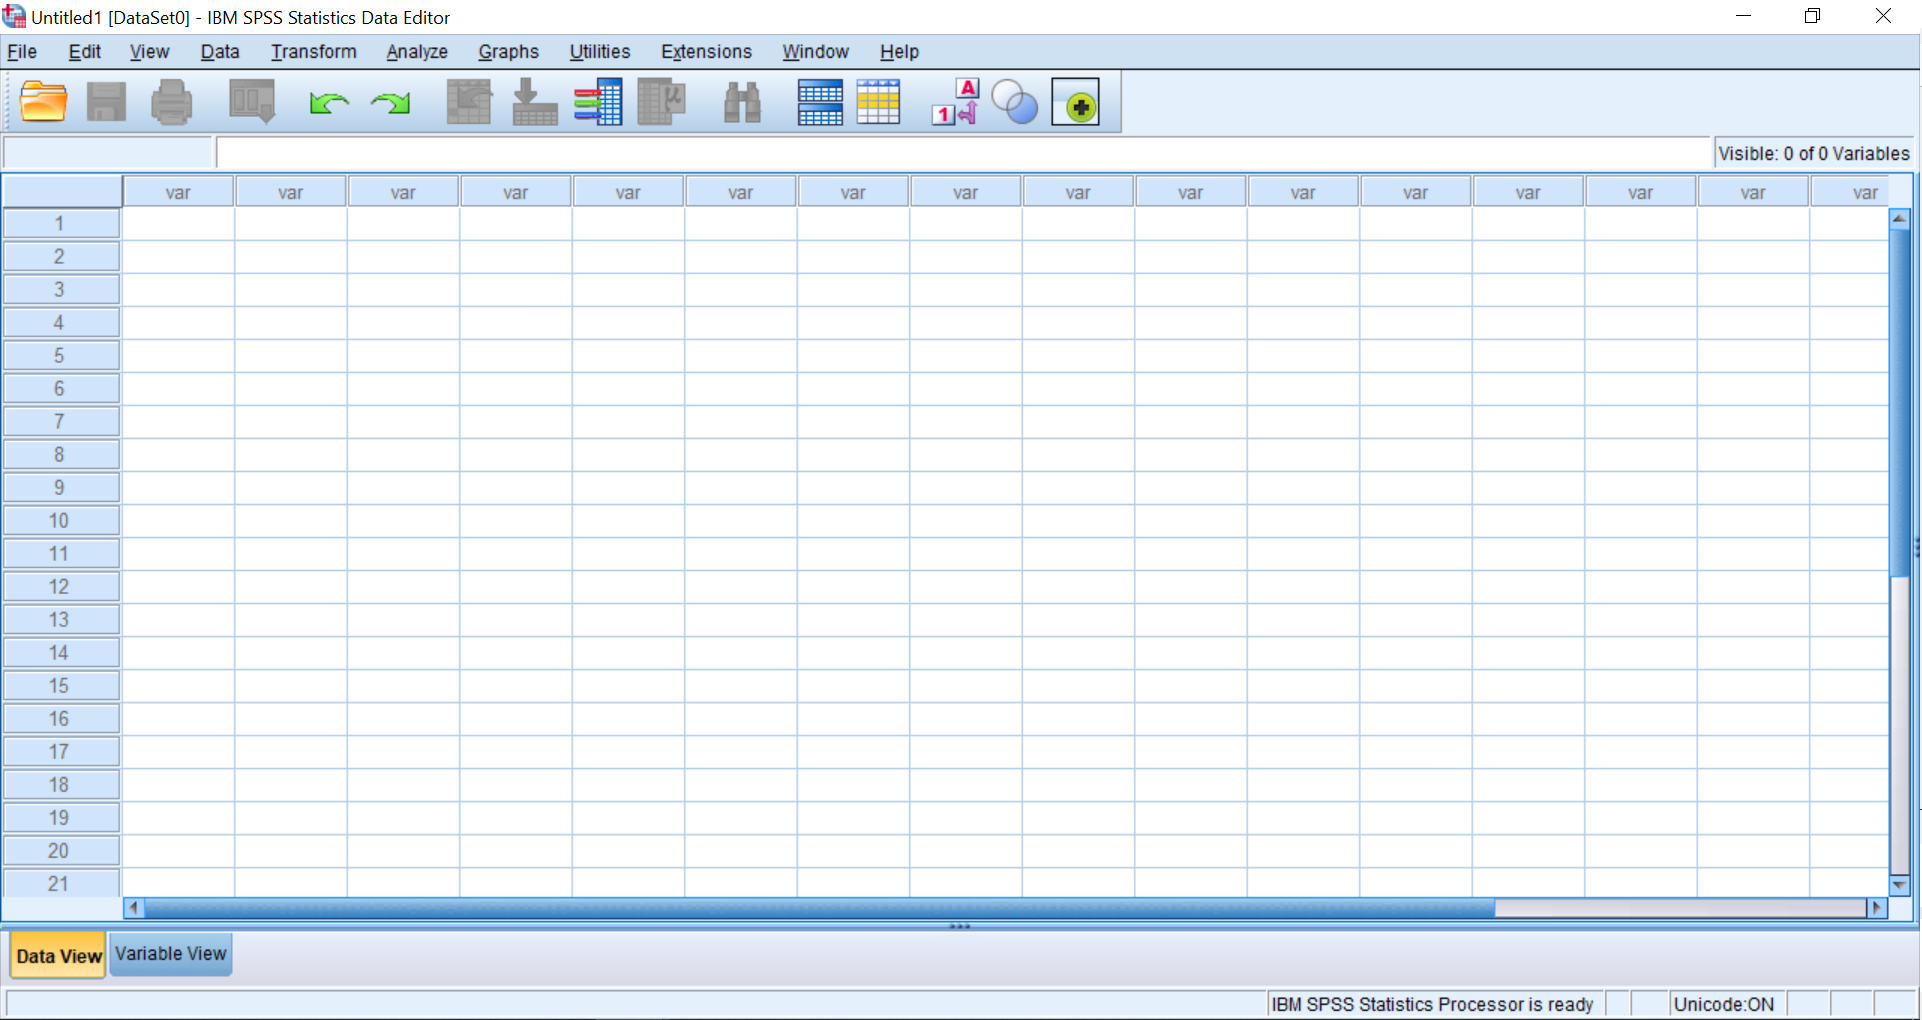
\includegraphics[width=12cm]{img/data_v1}
	\end{figure}
\end{frame}
%slide
\begin{frame}[t]{Reading IBM SPSS Statistics Data Files (Con..)}
	From the menus choose:\\
	\begin{itemize}
		\item File \textgreater Open \textgreater Data...\\
		\item Browse to and open demo.sav.\\
	\end{itemize}	
\end{frame}
%slide
\begin{frame}[t]{Reading IBM SPSS Statistics Data Files (Con..)}
	\begin{figure}
		\centering
		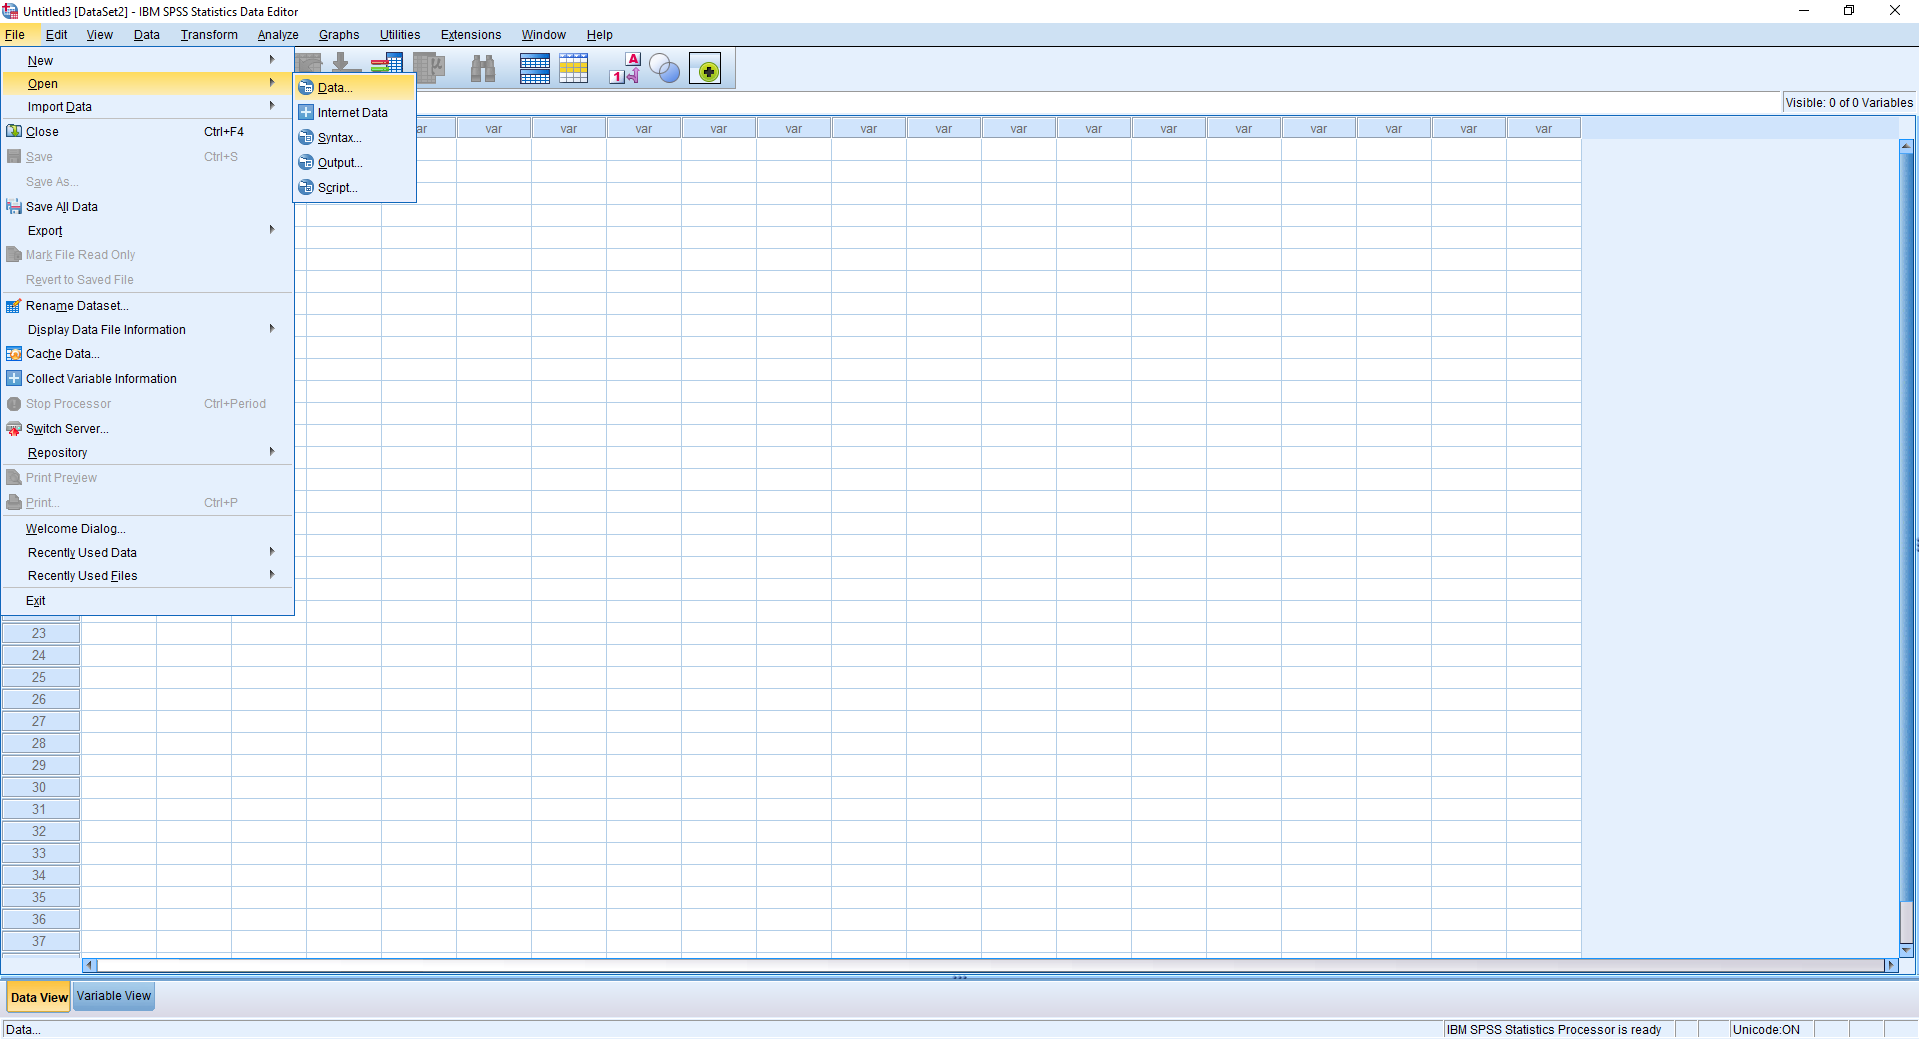
\includegraphics[width=12cm]{img/sav_data_1}
	\end{figure}
\end{frame}
%slide
\begin{frame}[t]{Reading IBM SPSS Statistics Data Files}
	\begin{figure}
		\centering
		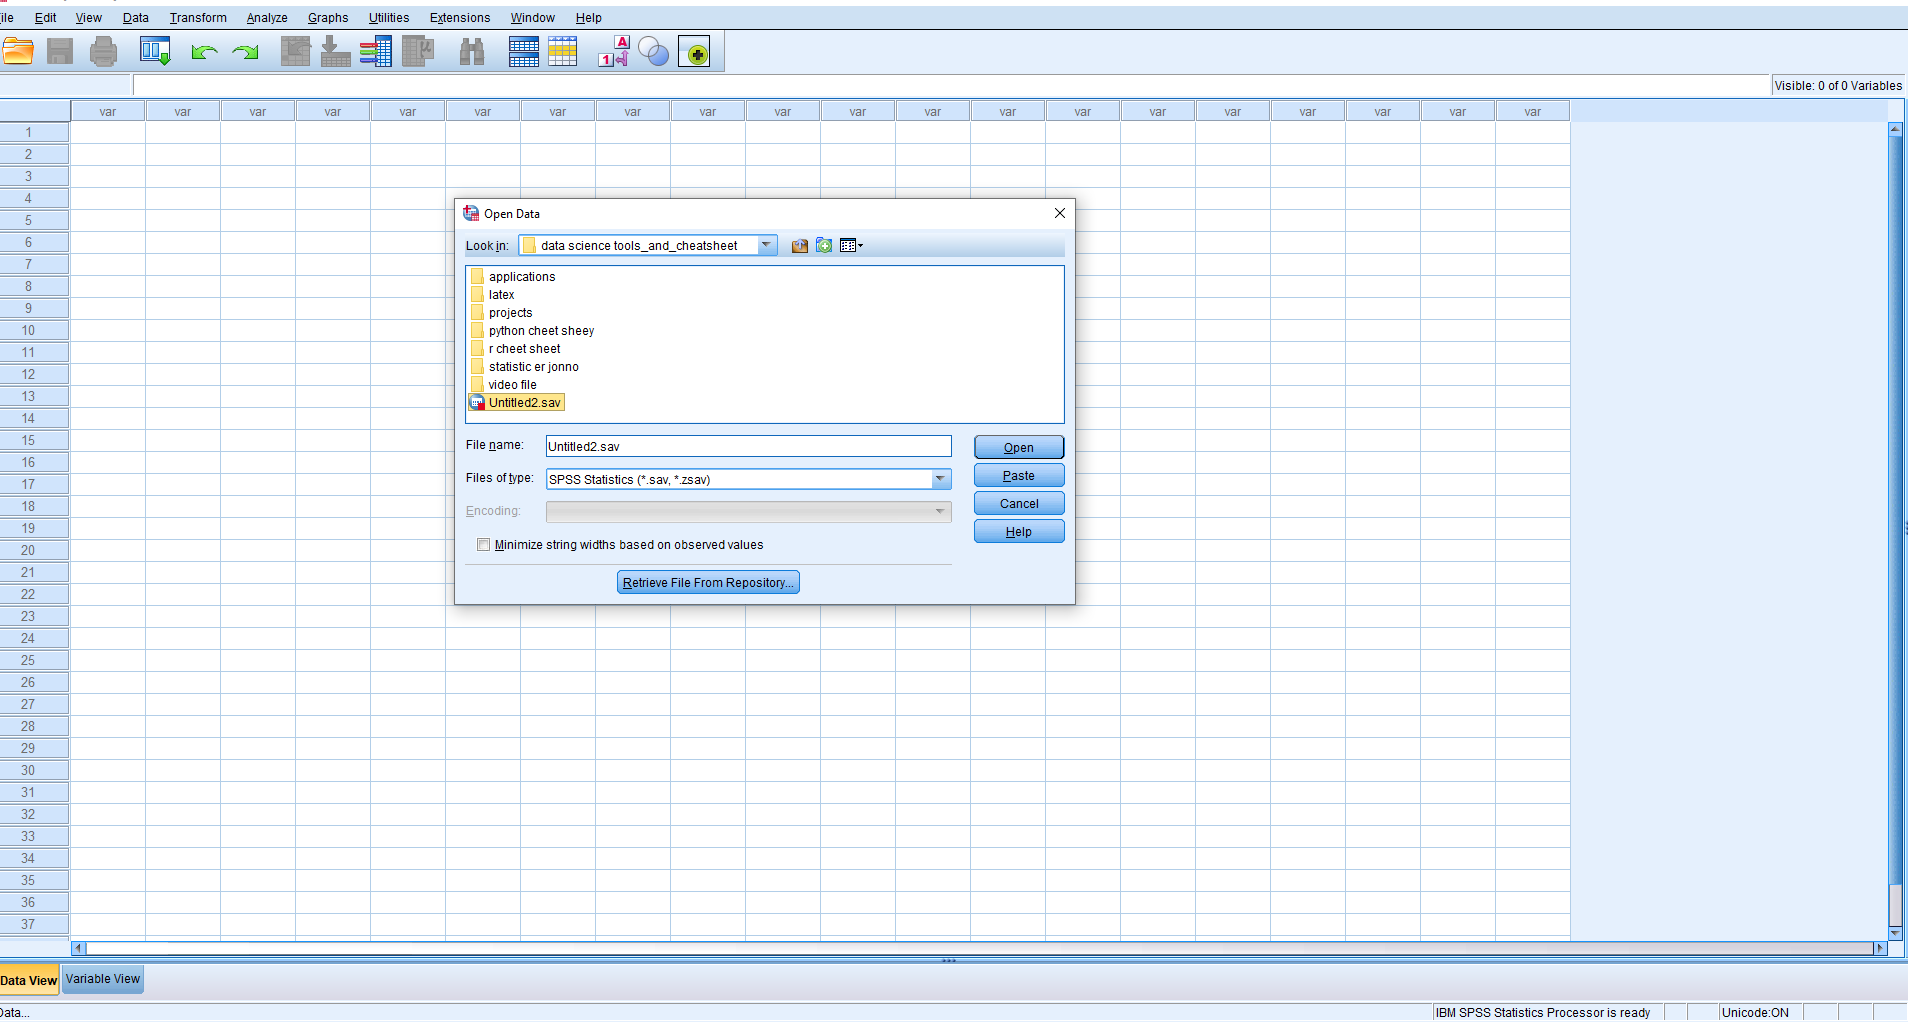
\includegraphics[width=12cm]{img/sav_data_2}
		\caption{Select Data file from directory}
	\end{figure}
\end{frame}
%slide
\begin{frame}[t]{Reading Data from Spreadsheets (Con..)}
	From the menus choose:\\
	\begin{itemize}
		\item 	File \textgreater Open \textgreater Data...\\
		\item Browse to and open demo.xls.\\
		\item Make sure that Read variable names from the first row of data is selected.\\
		\item Click OK to read the Excel file.\\
	\end{itemize}
\end{frame}
%slide
\begin{frame}[t]{Reading Data from Spreadsheets (Con..)}
	\begin{figure}
		\centering
		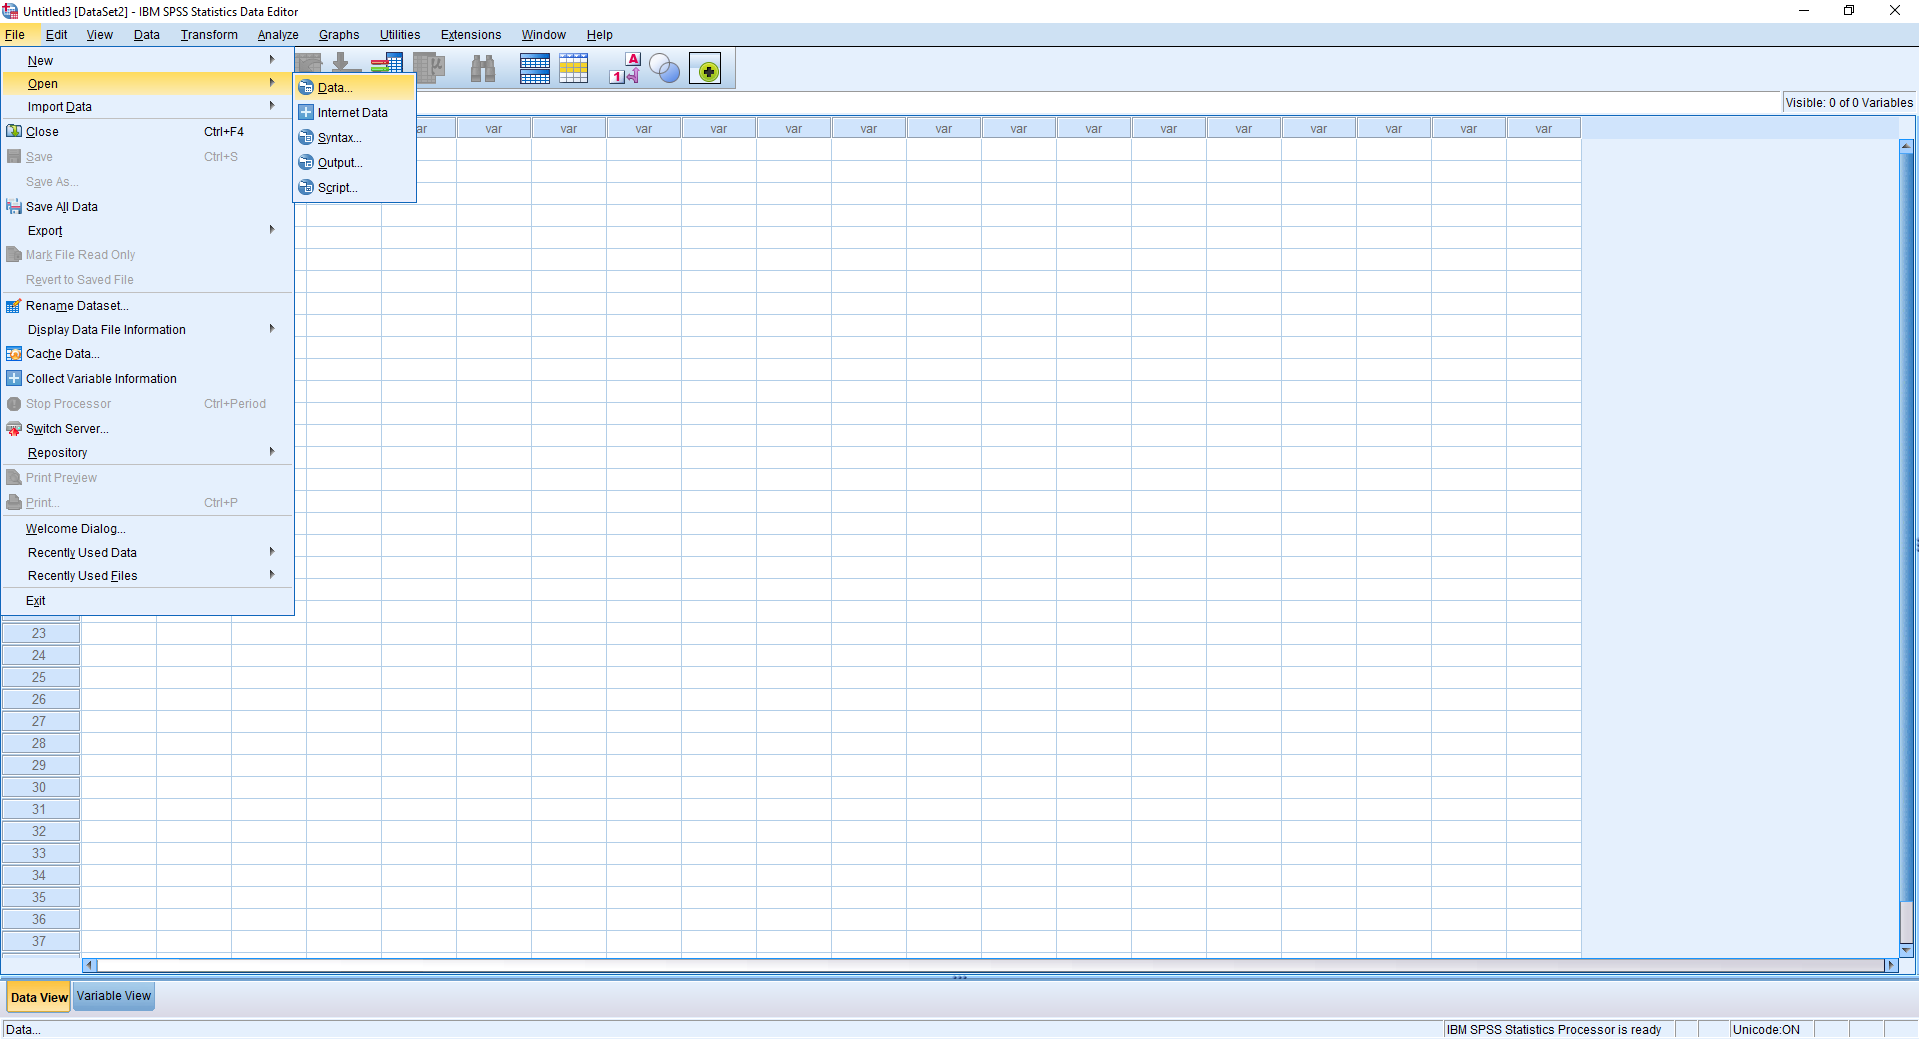
\includegraphics[width=12cm]{img/sav_data_1}
		\caption{1st step}
	\end{figure}
\end{frame}
%slide
\begin{frame}[t]{Reading Data from Spreadsheets}
	\begin{figure}
		\centering
		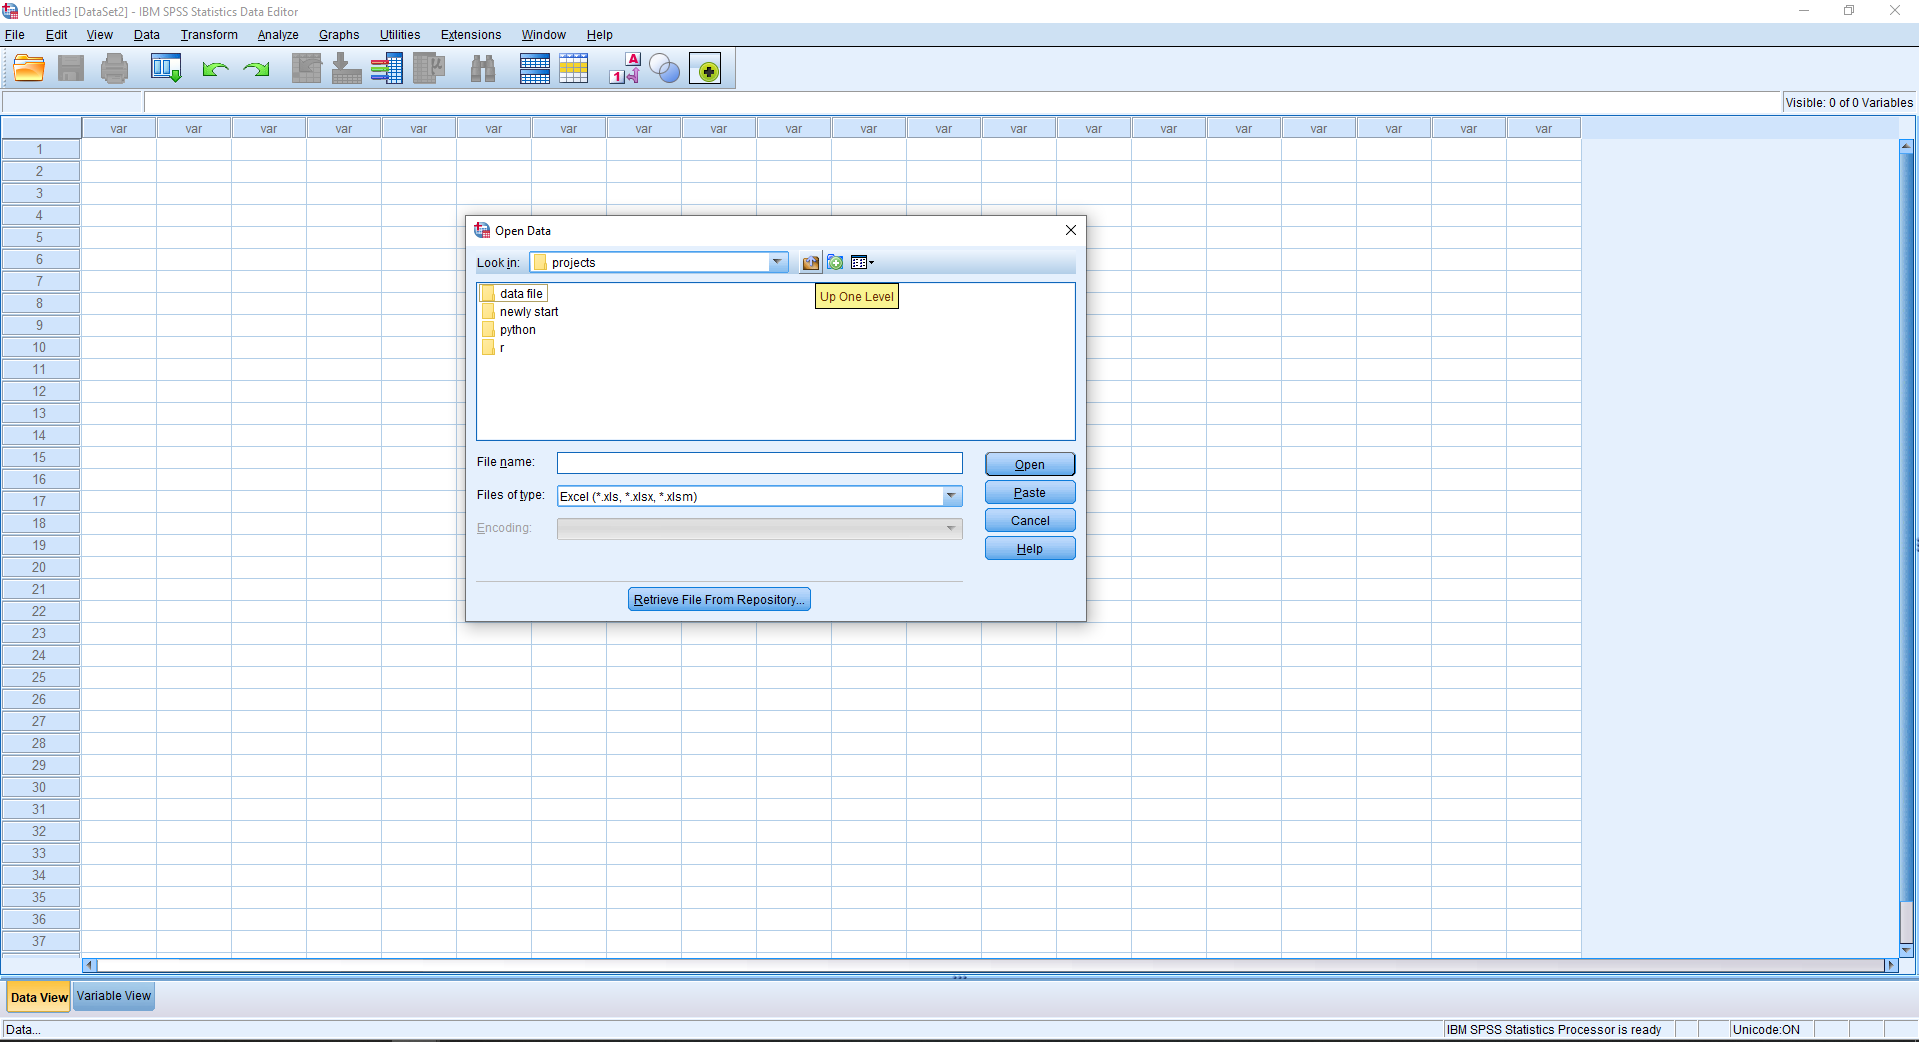
\includegraphics[width=12cm]{img/xls_data_1}
		\caption{1st step}
	\end{figure}
\end{frame}
%slide
\begin{frame}[t]{Reading Data from Others}
	Reading data from others source like - csv,database and text file is same as spreadsheets, SPSS files.
\end{frame}



% Sectuion Title 
\section{SECTION--III Create or Edit Dataset Using the Data Editor}
%slide
\begin{frame}[t]{Entering Numeric Data/ Creating Dataset (Con..)}
\begin{itemize}
	\item Click the Variable View tab at the bottom of the Data Editor window.
	\begin{figure}
		\centering
		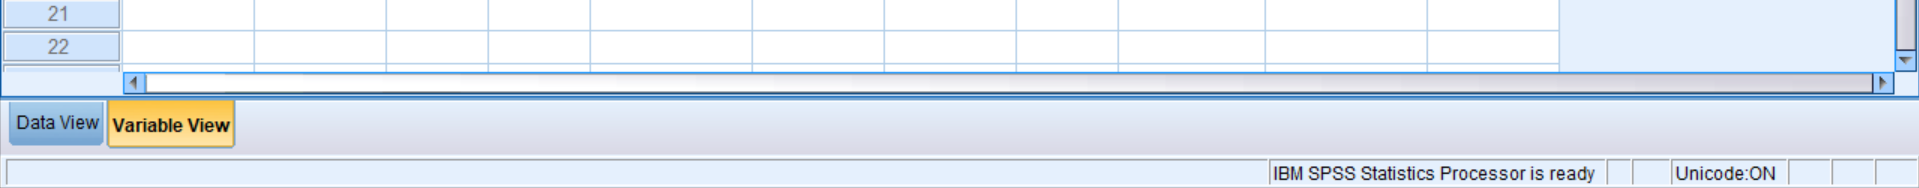
\includegraphics[width= 12cm]{img/variable_v1}
	\end{figure}
	\item In the first row of the first column, type age.
	\item In the second row, type marital.
	\item In the third row, type income.
\end{itemize}
\end{frame}
%slide
\begin{frame}[t]{Entering Numeric Data/ Creating Dataset (Con..)}
		\begin{figure}
		\centering
		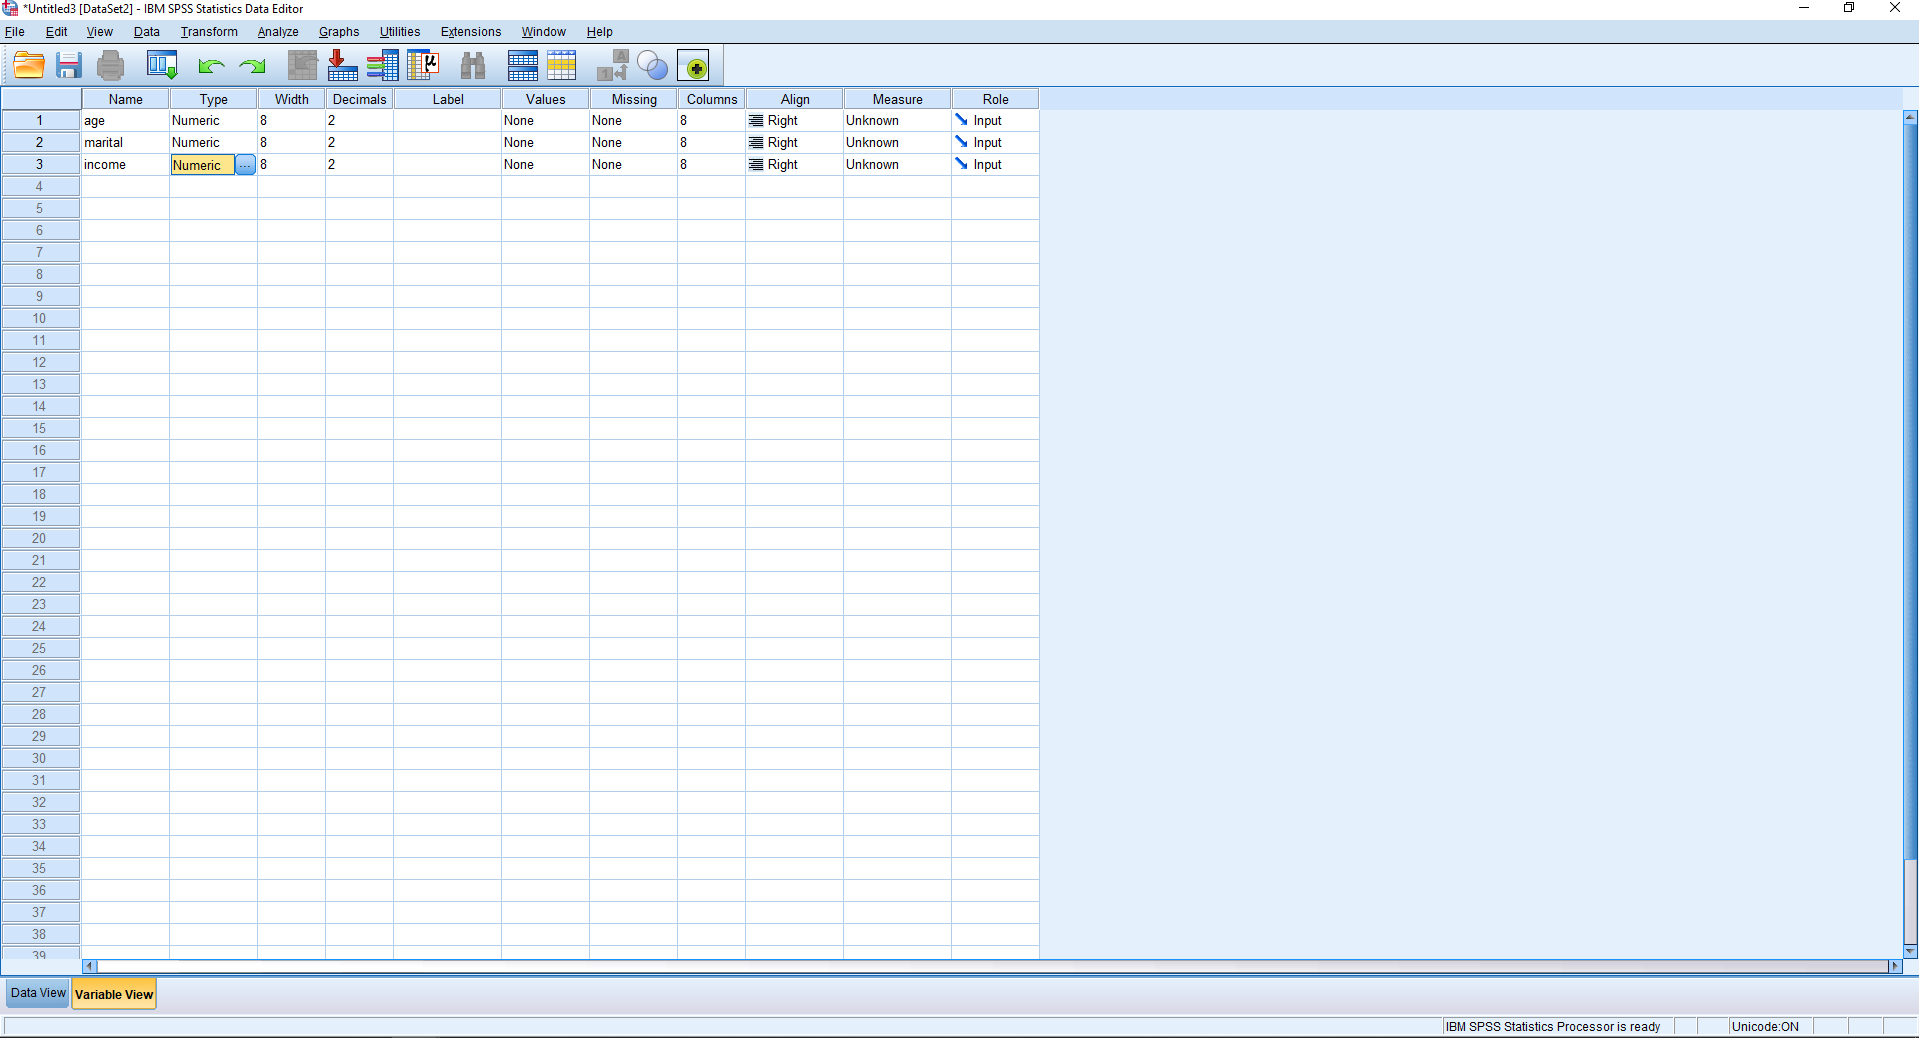
\includegraphics[width= 12cm]{img/variable_v2}
		\caption{Select Numeric Data Type}
	\end{figure}
\end{frame}
%slide
\begin{frame}[t]{Entering Numeric Data/ Creating Dataset (Con..)}
	\begin{itemize}
		\item Click the Data View tab to continue entering the data.
		\begin{figure}
			\centering
			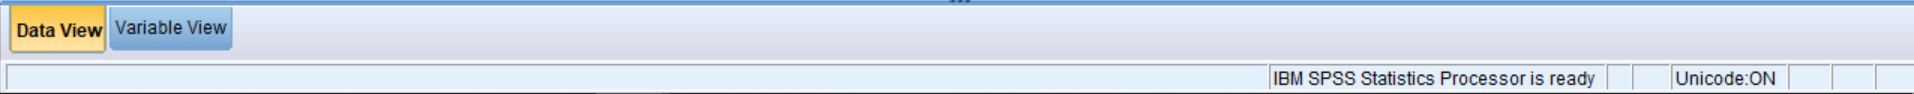
\includegraphics[width= 12cm]{img/data_v2}
		\end{figure}
		\item In the age column, type 55.
		\item In the marital column, type 1.
		\item In the income column, type 72000.
	\end{itemize}
\end{frame}
%slide
\begin{frame}[t]{Entering Numeric Data/ Creating Dataset}
	\begin{figure}
		\centering
		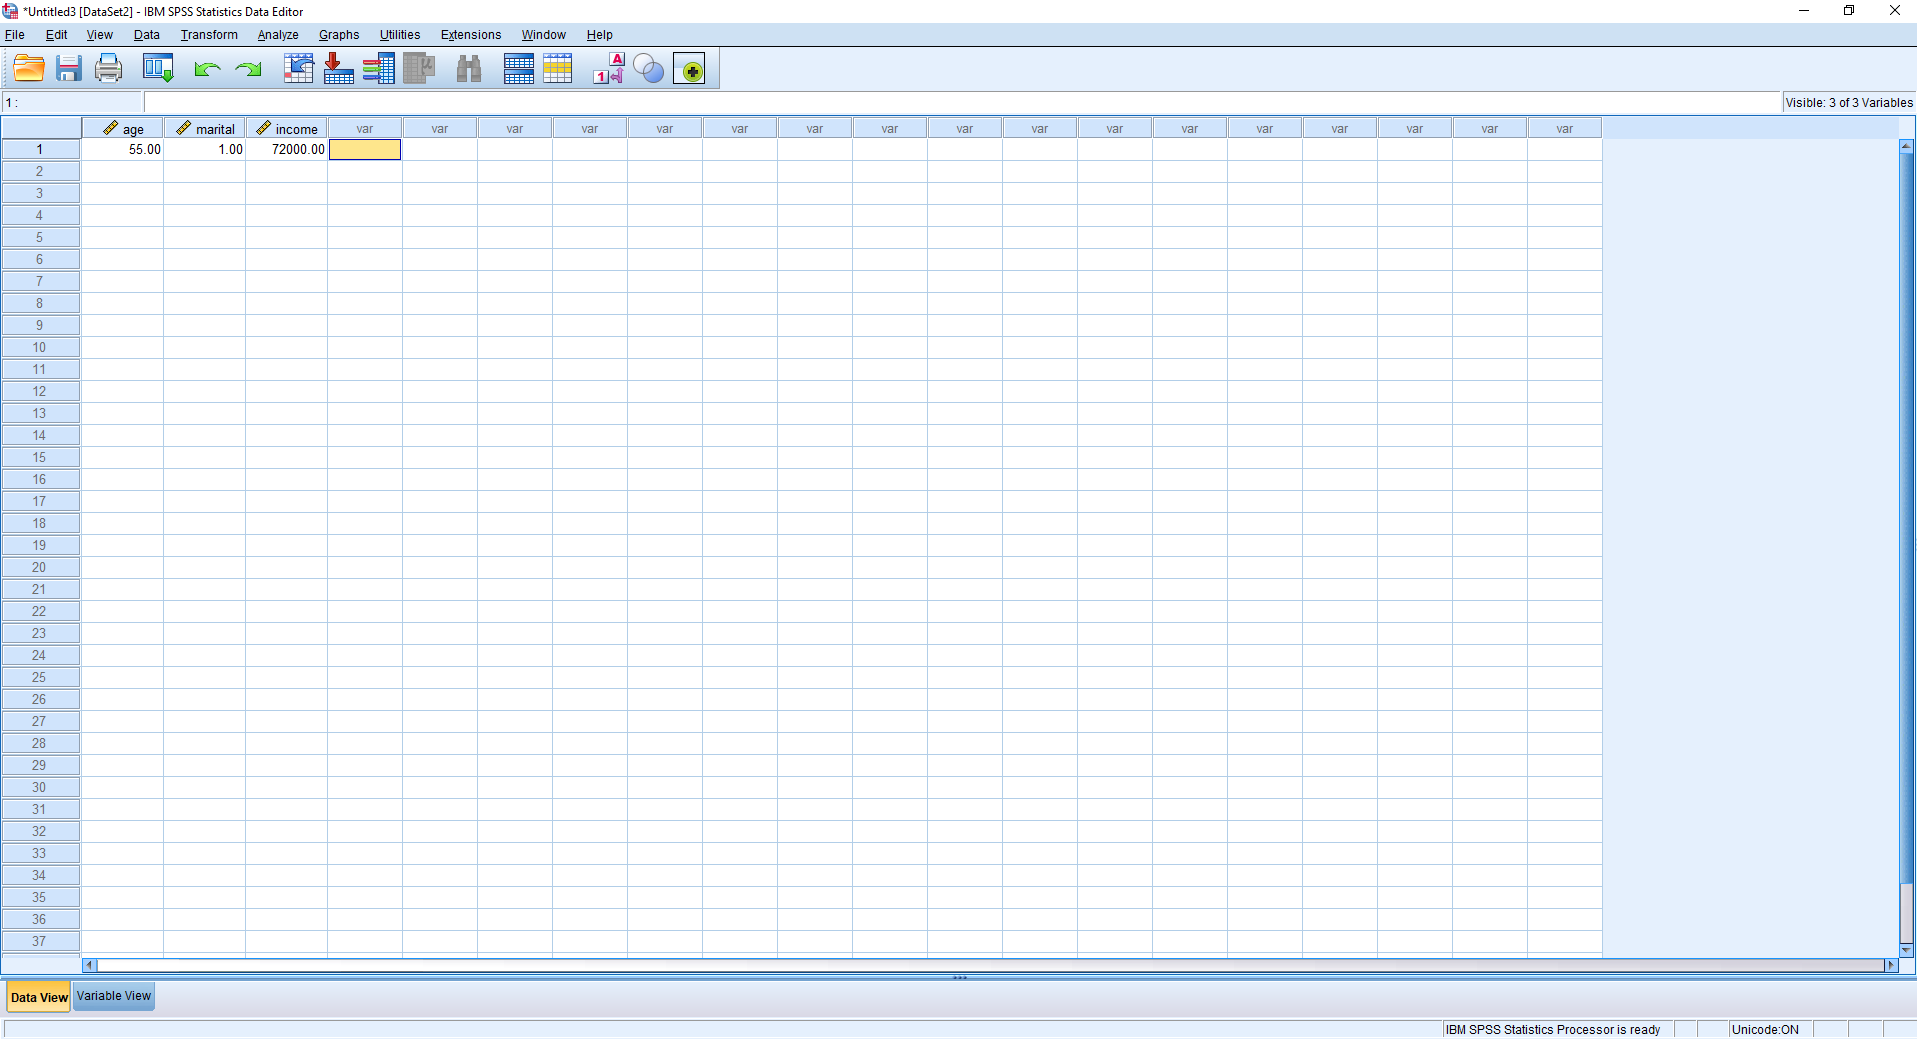
\includegraphics[width= 12cm]{img/enter_data_1}
		\caption{Numeric Data Entry}
	\end{figure}
\end{frame}



%slide
\begin{frame}[t]{Entering String Data (Con..)}
	\begin{itemize}
		\item Click the Variable View tab at the bottom of the Data Editor window.
		\item In the first cell of the first empty row, type name for the variable name.
		\item Click the Type cell next to your entry.
		
		\item Click the button on the right side of the Type cell to open the Variable Type dialog box.
		\item Select String to specify the variable type.
		\item Click OK to save your selection and return to the Data Editor.
	\end{itemize}
\end{frame}
%slide
\begin{frame}[t]{Entering String Data (Con..)}
	\begin{figure}
		\centering
		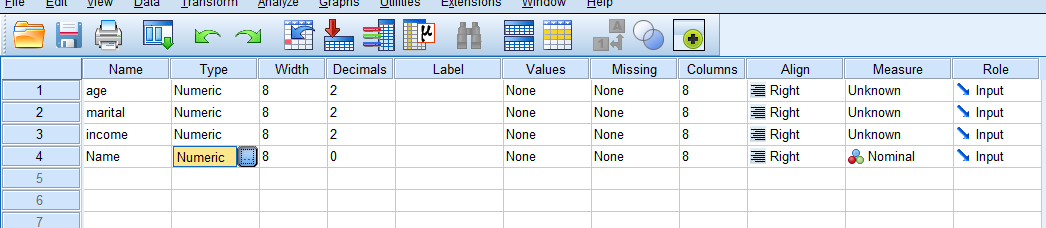
\includegraphics[width=14cm]{img/string_data_1}
		\caption{Click on Three Dots}
	\end{figure}
\end{frame}
%slide
\begin{frame}[t]{Entering String Data}
	\begin{figure}
		\centering
		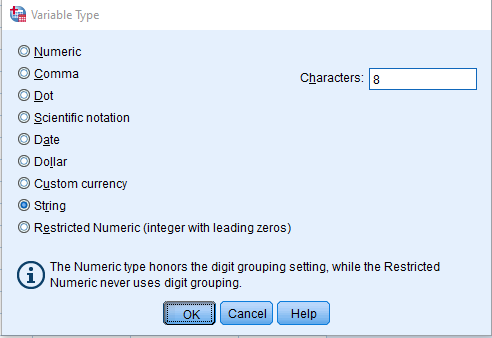
\includegraphics[width=9cm]{img/string_data_2}
		\caption{Select Variable Type}
	\end{figure}
\end{frame}



%slide
\begin{frame}[t]{Adding Variable Labels (Con..)}
	\begin{itemize}
		\item Click the Variable View tab at the bottom of the Data Editor window.
		\item In the Label column of the age row, type Respondent's Age.
		\item In the Label column of the marital row, type Marital Status.
		\item In the Label column of the income row, type Household Income.
		\item In the Label column of the name row, type Respondent's Name.
	\end{itemize}
\end{frame}
%slide
\begin{frame}[t]{Adding Variable Labels}
	\begin{figure}
	\centering
	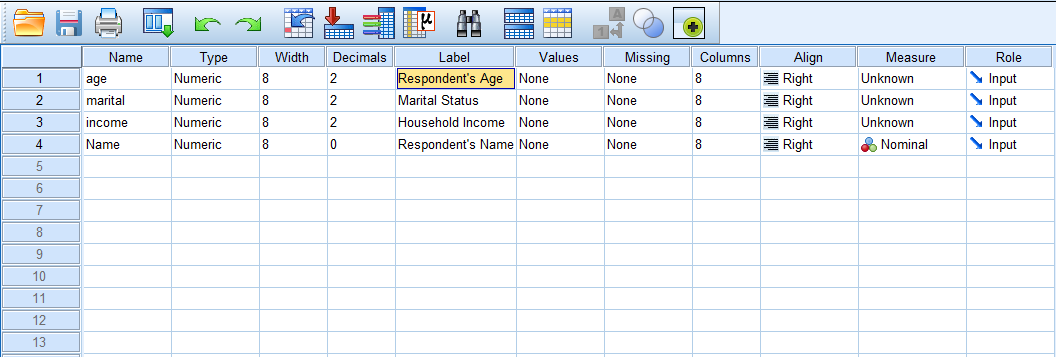
\includegraphics[width=14cm]{img/labeling}
	\caption{Labeling Variable}
	\end{figure}
\end{frame}
%slide
\begin{frame}[t]{Adding Value Labels for Numeric Variables and String Variables (Con..)}
	\begin{itemize}
		\item Click the Variable View tab at the bottom of the Data Editor window.Create a new variable - sex and it's \textbf{Label} is \textbf{Gender} and \textbf{Type} is \textbf{String}.
		
		\item Click the Values cell in the sex row, and then click the button on the right side of the cell to open the \textbf{Value Labels} dialog box.\\
		Type F in the Value field, and then type Female in the Label field.\\
		Type M in the Value field, and then type Male in the Label Field.
		
		\item Or for marital row -\\
		The \textbf{value label} is the string label that is applied to the specified numeric value.\\
		Type 0 in the Value field.\\
		Type Single in the Label field.
	\end{itemize}
\end{frame}
%slide
\begin{frame}[t]{Adding Value Labels for Numeric Variables and String Variables (Con..)}
	\begin{figure}
		\centering
		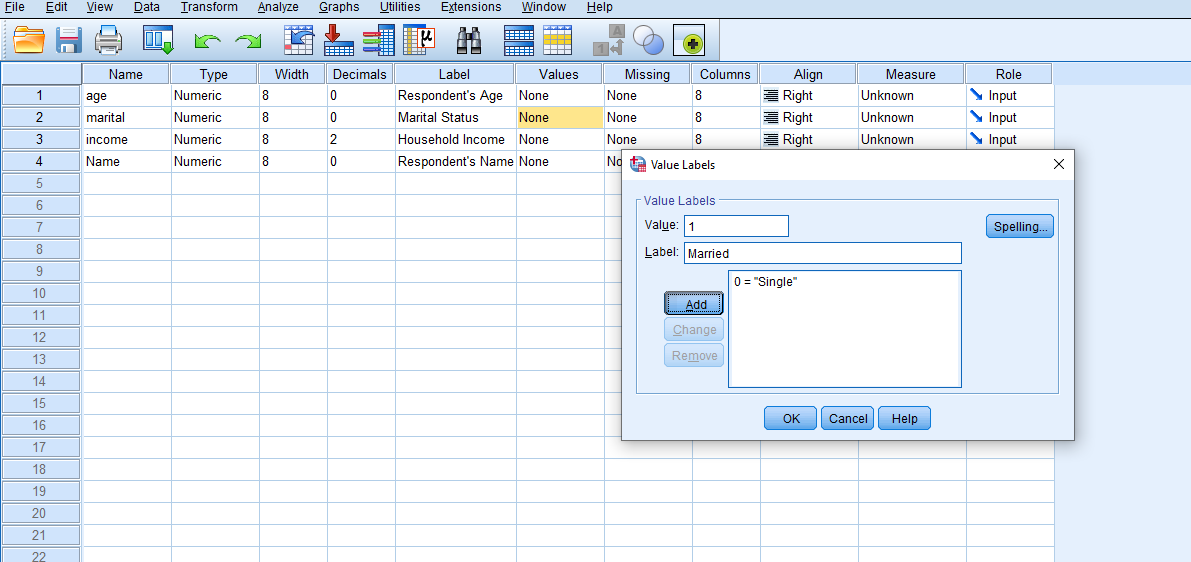
\includegraphics[width=12cm]{img/value_num}
		\caption{Numeric Variable}
	\end{figure}
\end{frame}
%slide
\begin{frame}[t]{Adding Value Labels for Numeric Variables and String Variables}
	\begin{figure}
		\centering
		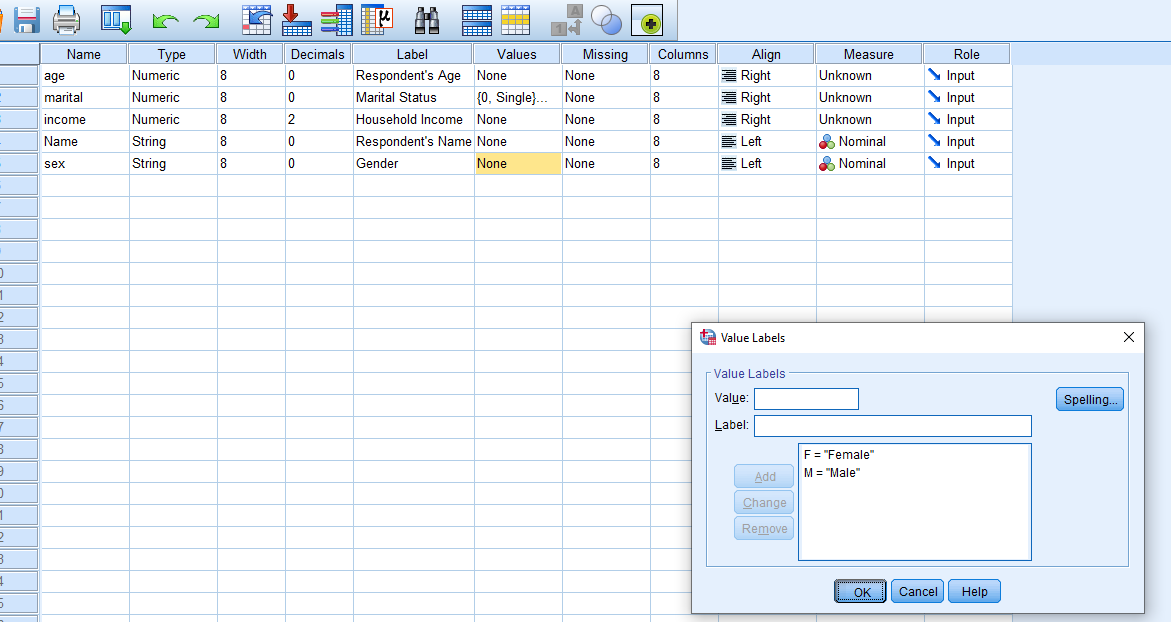
\includegraphics[width=12cm]{img/value_str}
		\caption{String Variable}
	\end{figure}
\end{frame}

%slide
%\begin{frame}
	%content...
%\end{frame}
% Thank you slide 
\plain{Thank You\\ \ \\ \Huge{\smiley}}

\end{document}